% Options for packages loaded elsewhere
\PassOptionsToPackage{unicode}{hyperref}
\PassOptionsToPackage{hyphens}{url}
%
\documentclass[
]{book}
\usepackage{amsmath,amssymb}
\usepackage{iftex}
\ifPDFTeX
  \usepackage[T1]{fontenc}
  \usepackage[utf8]{inputenc}
  \usepackage{textcomp} % provide euro and other symbols
\else % if luatex or xetex
  \usepackage{unicode-math} % this also loads fontspec
  \defaultfontfeatures{Scale=MatchLowercase}
  \defaultfontfeatures[\rmfamily]{Ligatures=TeX,Scale=1}
\fi
\usepackage{lmodern}
\ifPDFTeX\else
  % xetex/luatex font selection
\fi
% Use upquote if available, for straight quotes in verbatim environments
\IfFileExists{upquote.sty}{\usepackage{upquote}}{}
\IfFileExists{microtype.sty}{% use microtype if available
  \usepackage[]{microtype}
  \UseMicrotypeSet[protrusion]{basicmath} % disable protrusion for tt fonts
}{}
\makeatletter
\@ifundefined{KOMAClassName}{% if non-KOMA class
  \IfFileExists{parskip.sty}{%
    \usepackage{parskip}
  }{% else
    \setlength{\parindent}{0pt}
    \setlength{\parskip}{6pt plus 2pt minus 1pt}}
}{% if KOMA class
  \KOMAoptions{parskip=half}}
\makeatother
\usepackage{xcolor}
\usepackage{color}
\usepackage{fancyvrb}
\newcommand{\VerbBar}{|}
\newcommand{\VERB}{\Verb[commandchars=\\\{\}]}
\DefineVerbatimEnvironment{Highlighting}{Verbatim}{commandchars=\\\{\}}
% Add ',fontsize=\small' for more characters per line
\usepackage{framed}
\definecolor{shadecolor}{RGB}{248,248,248}
\newenvironment{Shaded}{\begin{snugshade}}{\end{snugshade}}
\newcommand{\AlertTok}[1]{\textcolor[rgb]{0.94,0.16,0.16}{#1}}
\newcommand{\AnnotationTok}[1]{\textcolor[rgb]{0.56,0.35,0.01}{\textbf{\textit{#1}}}}
\newcommand{\AttributeTok}[1]{\textcolor[rgb]{0.13,0.29,0.53}{#1}}
\newcommand{\BaseNTok}[1]{\textcolor[rgb]{0.00,0.00,0.81}{#1}}
\newcommand{\BuiltInTok}[1]{#1}
\newcommand{\CharTok}[1]{\textcolor[rgb]{0.31,0.60,0.02}{#1}}
\newcommand{\CommentTok}[1]{\textcolor[rgb]{0.56,0.35,0.01}{\textit{#1}}}
\newcommand{\CommentVarTok}[1]{\textcolor[rgb]{0.56,0.35,0.01}{\textbf{\textit{#1}}}}
\newcommand{\ConstantTok}[1]{\textcolor[rgb]{0.56,0.35,0.01}{#1}}
\newcommand{\ControlFlowTok}[1]{\textcolor[rgb]{0.13,0.29,0.53}{\textbf{#1}}}
\newcommand{\DataTypeTok}[1]{\textcolor[rgb]{0.13,0.29,0.53}{#1}}
\newcommand{\DecValTok}[1]{\textcolor[rgb]{0.00,0.00,0.81}{#1}}
\newcommand{\DocumentationTok}[1]{\textcolor[rgb]{0.56,0.35,0.01}{\textbf{\textit{#1}}}}
\newcommand{\ErrorTok}[1]{\textcolor[rgb]{0.64,0.00,0.00}{\textbf{#1}}}
\newcommand{\ExtensionTok}[1]{#1}
\newcommand{\FloatTok}[1]{\textcolor[rgb]{0.00,0.00,0.81}{#1}}
\newcommand{\FunctionTok}[1]{\textcolor[rgb]{0.13,0.29,0.53}{\textbf{#1}}}
\newcommand{\ImportTok}[1]{#1}
\newcommand{\InformationTok}[1]{\textcolor[rgb]{0.56,0.35,0.01}{\textbf{\textit{#1}}}}
\newcommand{\KeywordTok}[1]{\textcolor[rgb]{0.13,0.29,0.53}{\textbf{#1}}}
\newcommand{\NormalTok}[1]{#1}
\newcommand{\OperatorTok}[1]{\textcolor[rgb]{0.81,0.36,0.00}{\textbf{#1}}}
\newcommand{\OtherTok}[1]{\textcolor[rgb]{0.56,0.35,0.01}{#1}}
\newcommand{\PreprocessorTok}[1]{\textcolor[rgb]{0.56,0.35,0.01}{\textit{#1}}}
\newcommand{\RegionMarkerTok}[1]{#1}
\newcommand{\SpecialCharTok}[1]{\textcolor[rgb]{0.81,0.36,0.00}{\textbf{#1}}}
\newcommand{\SpecialStringTok}[1]{\textcolor[rgb]{0.31,0.60,0.02}{#1}}
\newcommand{\StringTok}[1]{\textcolor[rgb]{0.31,0.60,0.02}{#1}}
\newcommand{\VariableTok}[1]{\textcolor[rgb]{0.00,0.00,0.00}{#1}}
\newcommand{\VerbatimStringTok}[1]{\textcolor[rgb]{0.31,0.60,0.02}{#1}}
\newcommand{\WarningTok}[1]{\textcolor[rgb]{0.56,0.35,0.01}{\textbf{\textit{#1}}}}
\usepackage{longtable,booktabs,array}
\usepackage{calc} % for calculating minipage widths
% Correct order of tables after \paragraph or \subparagraph
\usepackage{etoolbox}
\makeatletter
\patchcmd\longtable{\par}{\if@noskipsec\mbox{}\fi\par}{}{}
\makeatother
% Allow footnotes in longtable head/foot
\IfFileExists{footnotehyper.sty}{\usepackage{footnotehyper}}{\usepackage{footnote}}
\makesavenoteenv{longtable}
\usepackage{graphicx}
\makeatletter
\def\maxwidth{\ifdim\Gin@nat@width>\linewidth\linewidth\else\Gin@nat@width\fi}
\def\maxheight{\ifdim\Gin@nat@height>\textheight\textheight\else\Gin@nat@height\fi}
\makeatother
% Scale images if necessary, so that they will not overflow the page
% margins by default, and it is still possible to overwrite the defaults
% using explicit options in \includegraphics[width, height, ...]{}
\setkeys{Gin}{width=\maxwidth,height=\maxheight,keepaspectratio}
% Set default figure placement to htbp
\makeatletter
\def\fps@figure{htbp}
\makeatother
\setlength{\emergencystretch}{3em} % prevent overfull lines
\providecommand{\tightlist}{%
  \setlength{\itemsep}{0pt}\setlength{\parskip}{0pt}}
\setcounter{secnumdepth}{5}
\usepackage{booktabs} 
\ifLuaTeX
  \usepackage{selnolig}  % disable illegal ligatures
\fi
\usepackage[]{natbib}
\bibliographystyle{apalike}
\usepackage{bookmark}
\IfFileExists{xurl.sty}{\usepackage{xurl}}{} % add URL line breaks if available
\urlstyle{same}
\hypersetup{
  pdftitle={A protocol for sequencing and analysing 16S-ITS-23S amplicons using Oxford Nanopore's Native Barcoding kit to profile prokaryotes on species-level in a mixed community {[}Under development{]}},
  pdfauthor={Christian Krohn, PhD, RMIT University},
  hidelinks,
  pdfcreator={LaTeX via pandoc}}

\title{A protocol for sequencing and analysing 16S-ITS-23S amplicons using Oxford Nanopore's Native Barcoding kit to profile prokaryotes on species-level in a mixed community {[}Under development{]}}
\author{\href{https://www.rmit.edu.au/contact/staff-contacts/academic-staff/k/krohn---christian}{Christian Krohn, PhD, RMIT University}}
\date{2024-07-29}

\begin{document}
\maketitle

{
\setcounter{tocdepth}{1}
\tableofcontents
}
\chapter{About this GitBook}\label{about}

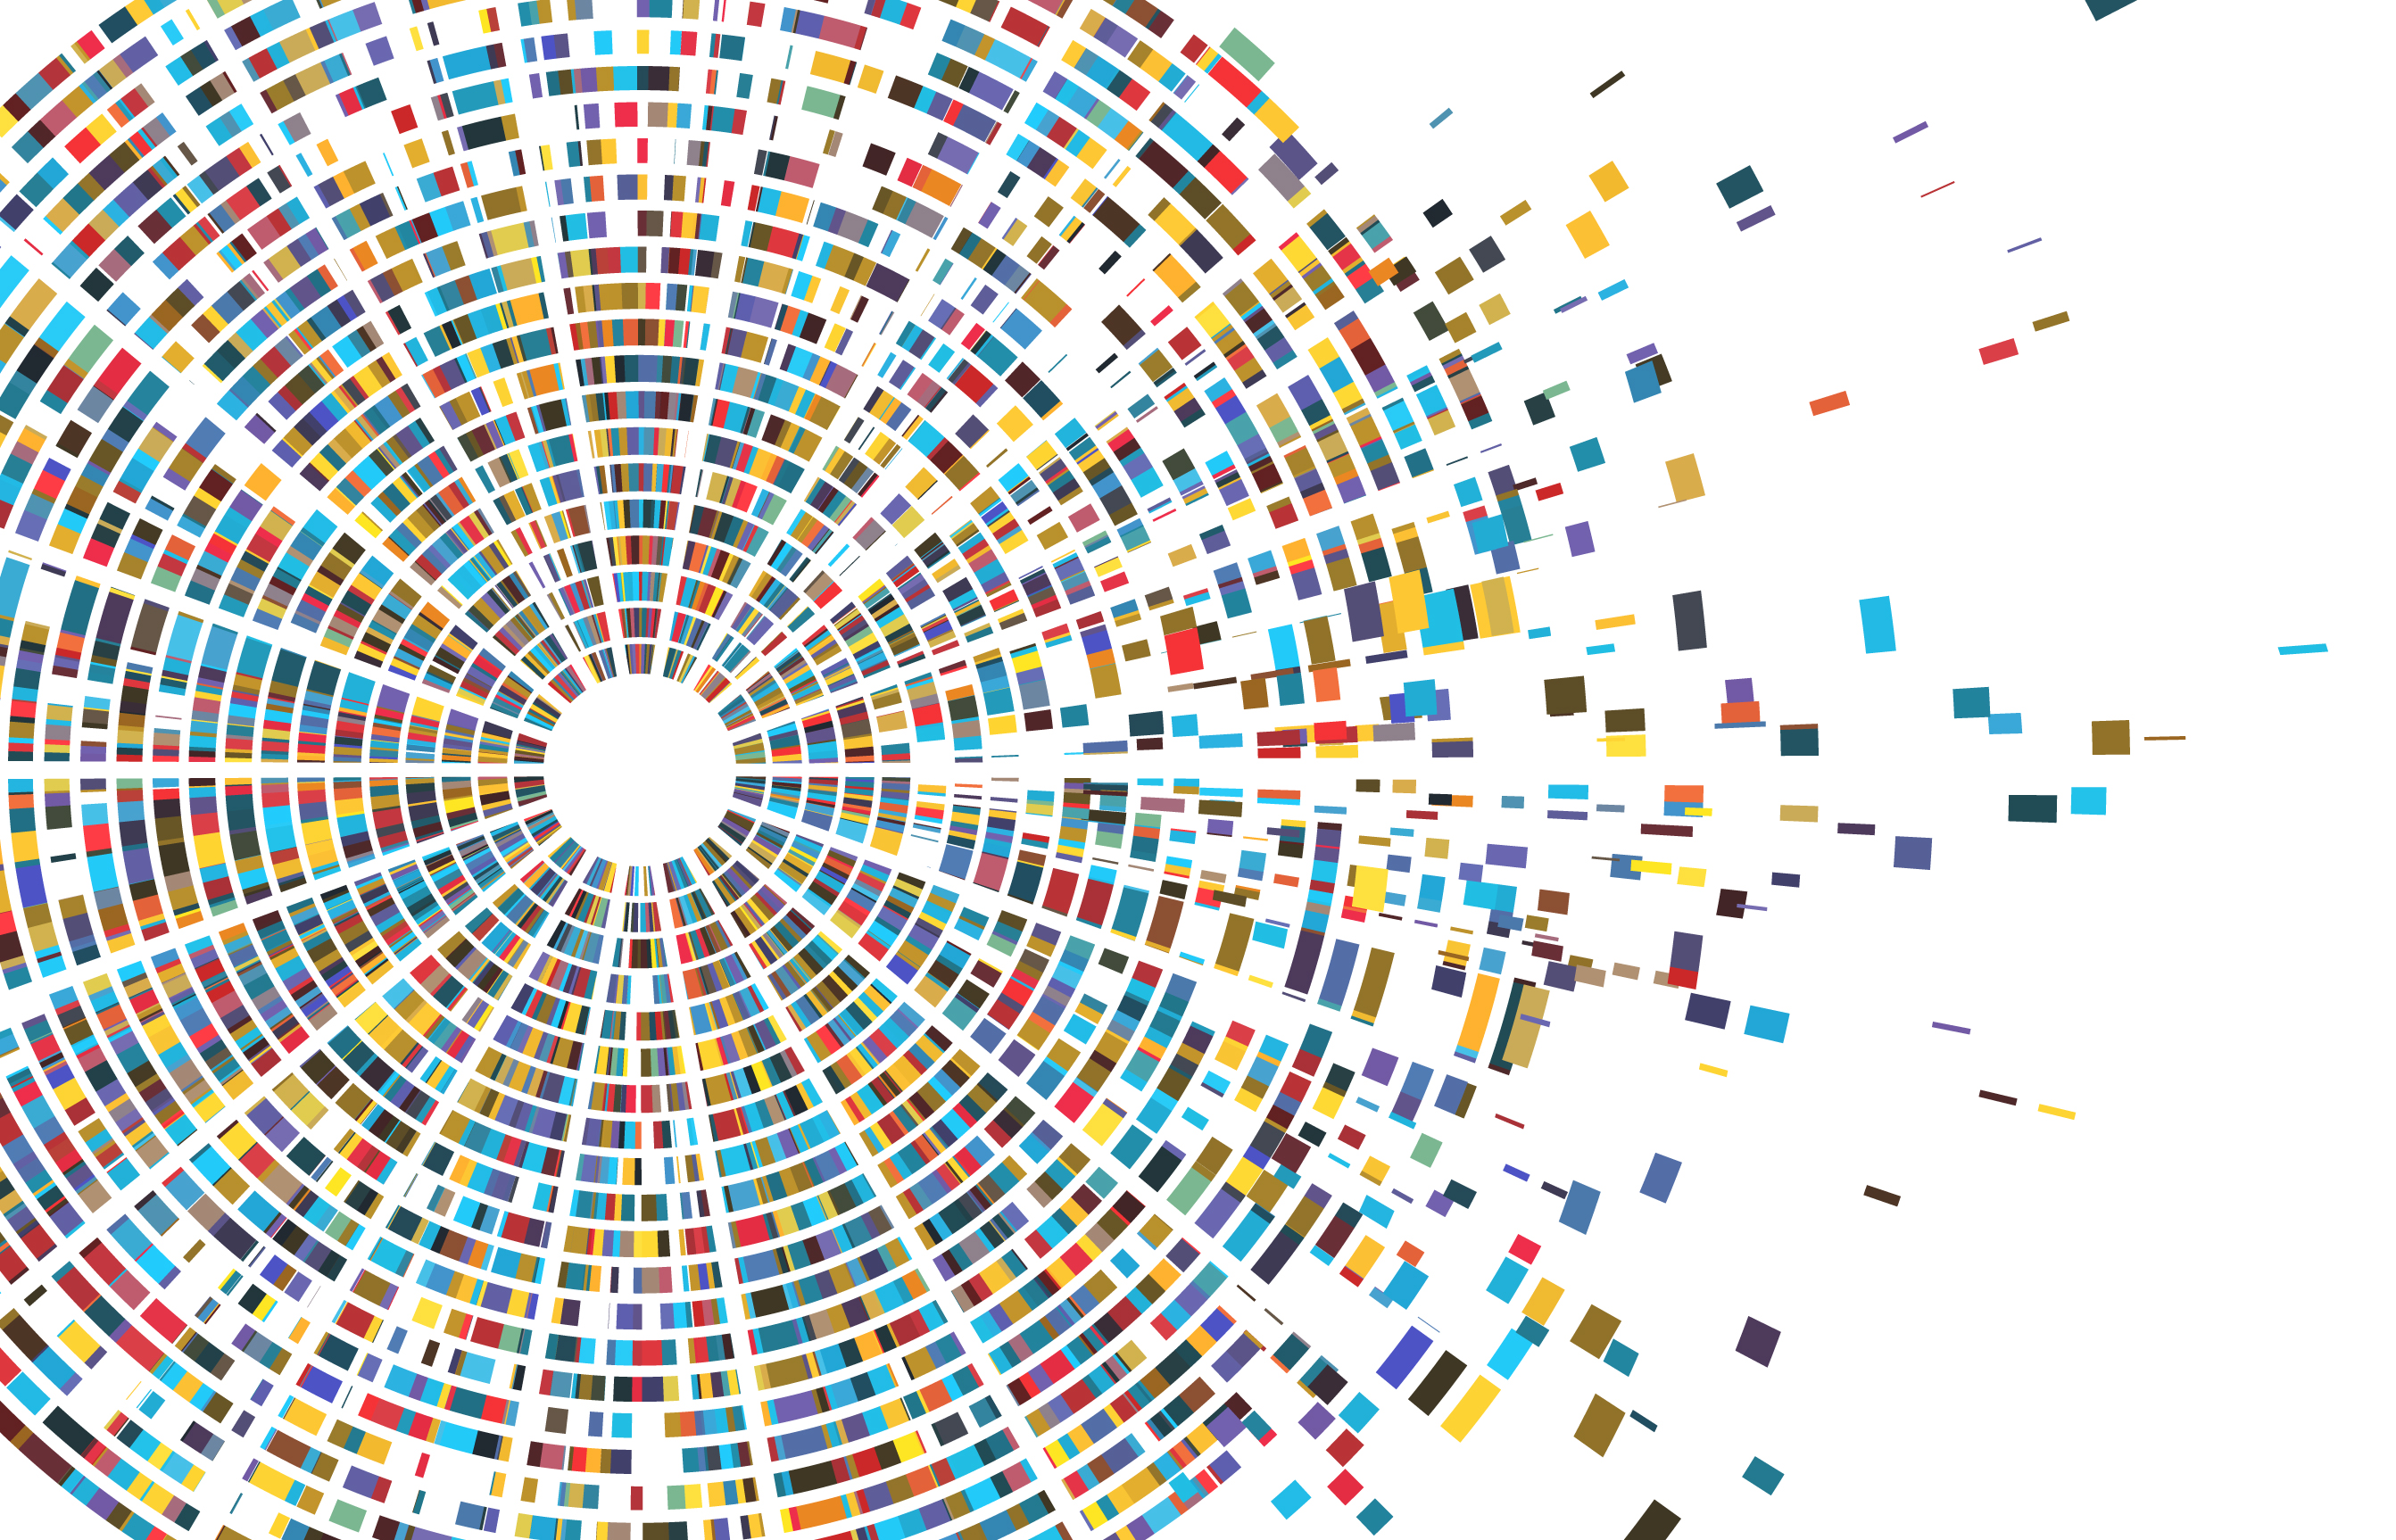
\includegraphics[width=5.20833in,height=\textheight]{./img/vectorstock_23650232.jpg}

This GitBook is under development (2024).

This GitBook provides a step-by-step protocol for anyone who want to get started with sequencing multiple samples of high quality, full-length microbial amplicons (16S-ITS-23S) with an Oxford Nanopore instrument, and then process and visualise the data using various packages in R. The aim is to profile a community of bacteria and archaea on \textbf{species-level}.

Read and use this protocol either directly or to develop your own.

This protocol reflects the experiences we had in the lab and may help to get you started on your own journey of discovery. One of the biggest hurdles is the effort required to learn new technologies, hence this protocol aims at lowering your `activation' energy by providing some guidance for each step from DNA extraction, to amplification, library preparation, sequencing, data processing and finally some basic visualisations in R.

This protocol uses the DNeasy Powersoil Pro Kit (Qiagen, Hilden, Germany) to extract DNA from wastewater sludge, as well as the Native Barcoding Kit (SQK-NBD114.96) with a R10.4.1 flowcell (FLO-MIN114) to sequence long (\textasciitilde4-4.4 kb) amplicons from environmental DNA. The primer used was developed by \citep{Martijn2019}. Initial costs to purchase all consumables will be \textasciitilde AUD\$7,700.

Check out our workflows for short-read 16S sequencing at \url{https://chrismitbiz.github.io/ABlab-workflows} if you want to get started with Miseq 16S sequencing instead.

If you are interested in sequencing the living biomass via PMA treatment in combination with short-read 16S sequencing, check out our recent paper \href{https://doi.org/10.1016/j.watres.2024.121354}{Dead in the water -- Role of relic DNA and primer choice for targeted sequencing surveys of anaerobic sewage sludge intended for biological monitoring} \citep{Krohn2024}

\textbf{Get in touch}

We work at the Andy Ball lab, RMIT University, Bundoora, Melbourne and are part of the Industry-led \href{https://www.transformingbiosolids.org.au}{Biosolids Training Centre}. Email me or comment on the discussion section of the \href{https://github.com/chrismitbiz/ABlab-workflows/discussions/}{GitHub repository} for this GitBook. You will need to get a GitHub account to join the discussion. Its free.

More about me and my PhD research can be found here: \url{https://clean-dirt-digests.netlify.app}.\\
Follow me on \href{https://twitter.com/CleanDirtChris}{X} (hardly use that anymore though) or \href{https://www.linkedin.com/in/christian-krohn-54904855}{LinkedIn}.

~

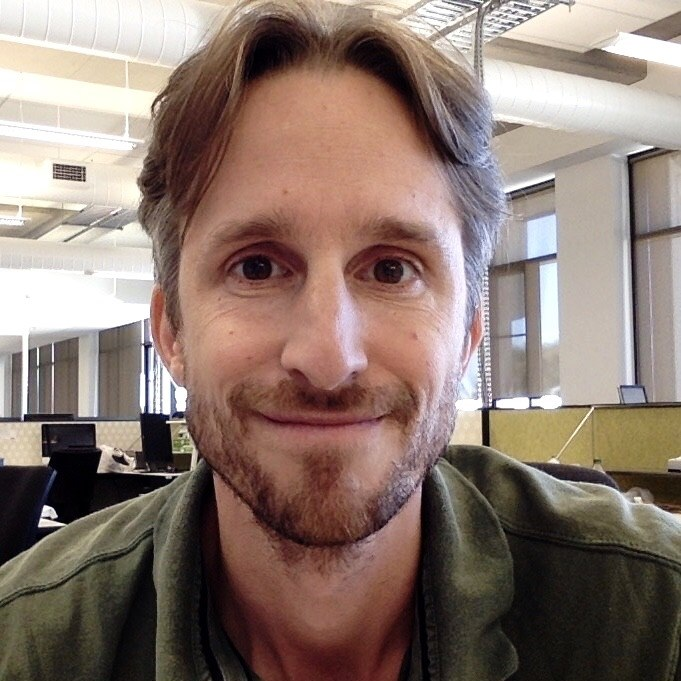
\includegraphics[width=1.5625in,height=\textheight]{./img/avatar.jpg}

Bio:\\
Dr Chris Krohn is an early career researcher whose interests could be summed up with: ``Environmental sequencing, microbial ecology, chlorinated pollutants, organic matter, wastewater, anaerobic digestion, and how everything connects''.

In 2021 I joined the ARC Biosolids Training Centre at RMIT (www.transformingbiosolids.org.au), where we help water utilities to improve circular resource management by getting more renewable biogas and carbon/fertiliser values out of our municipal biosolids (essentially our poo). In project 1C of the Centre I develop metagenomic (DNA-based) methods to monitor the microbiome of anaerobic digestion, an important microbial treatment process for wastewater. I believe DNA-based diagnoses of wastewater sludges will help the water/biosolids sector improve resource recoveries and risk management.

Before that, after a career in one of the most fast-cycled and short-sighted manufacturing industries that took me from Germany to Vietnam and Hong Kong/Shenzhen, I decided to hit the switch and start thinking long-term and circular. Ten back-to-uni years later, in 2021 I finished a PhD in Soil Science at La Trobe Uni where I sequenced soil DNA and explored if and how soil biology was involved in the degradation of extremely persistent legacy pesticides that contaminate agricultural surface soils since several decades.\\

This work is licensed under a Creative Commons Attribution 4.0 International License.

\chapter{Prerequisites, equipment and consumables}\label{prerequisites}

\section{Prerequisites}\label{prerequisites-1}

\begin{itemize}
\tightlist
\item
  Experience with basic molecular laboratory techniques and DNA quality control (use of laminar flow hood, pipetting micro volumes, handling and preserving small volume reagents, sterilisation of consumables, doing gel electrophoresis)
\item
  Experience with loading Nanopore flowcells

  \begin{itemize}
  \tightlist
  \item
    It is vital that loading of the flowcell is practiced.The key is to avoid any air entering the flow cell as that will completely destroy the pores. Use an old flowcell if available and run through the process with water to see where the buffers flow. Afterwards we recommend doing a Control run with Lambda DNA using the \href{https://store.nanoporetech.com/control-expansion.html}{Control Expansion Kit}).
  \end{itemize}
\item
  Confident with R, R Studio and package environment managers such as Conda and Docker. Knowledge in shell scripting and Linux syntax.
\end{itemize}

\section{DNA extraction kit}\label{dna-extraction-kit}

We commonly extract DNA from soils or from wastewater sludges using the DNeasy Powersoil Pro Kit (Qiagen) for both, soil and sludge. It resulted in high quality DNA, suitable for library preparation and sequencing. Extraction with this kit includes a bead beating step to release DNA from cells out of difficult matrices such as soils and sludge (biofilms) or similar. The sheared DNA will be fragmented with a N50 of \textasciitilde7 kb in some cases \citep{Jensen2024}. Shearing of DNA may be minimised by reducing/optimising bead-beating duration and speed. Other commonly used and commercially available kits for DNA extraction are available \citep{Jensen2024, Gand2023}.

\begin{figure}
\centering
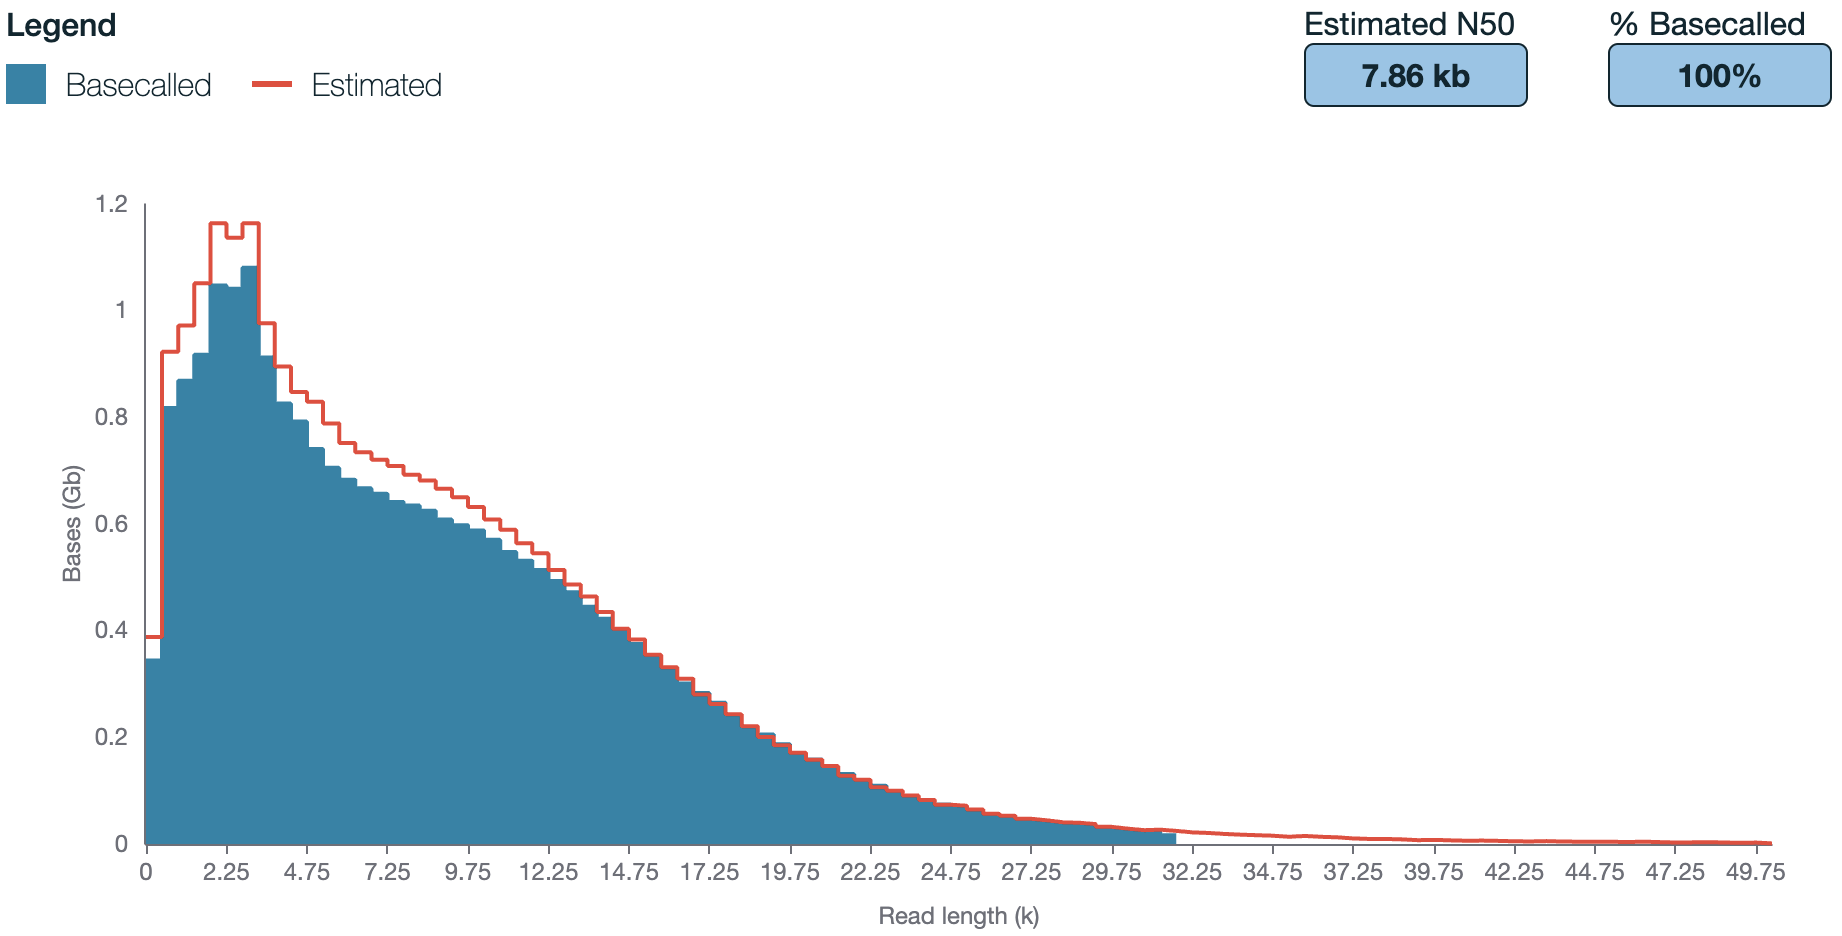
\includegraphics[width=6.25in,height=\textheight]{./img/readsize.png}
\caption{``Example of read size distribution of sludge DNA extracted with the DNeasy Powersoil Pro Kit in our lab''}
\end{figure}

\section{Other consumables}\label{other-consumables}

\begin{itemize}
\tightlist
\item
  Native Barcoding Kit (Oxford Nanopore, SQK-NBD114.96)\\
\item
  R10.4.1 flowcell (Oxford Nanopore, FLO-MIN114)
\item
  NEBNext Quick Ligation Module (E6056, New England Biolab)
\item
  NEBNext Ultra II End repair/dA-tailing Module (E7546S, New England Biolab)
\item
  Blunt/TA Ligase Master Mix (M0367, New England Biolab)
\item
  10 mM dNTPs (N0447S, New England Biolab)
\item
  Q5 Hot Start High-Fidelity DNA Polymerase (M0493, New England Biolab)
\item
  DNeasy Powersoil Pro Kit (\#47016, Qiagen)
\item
  Qubit 1X dsDNA BR or HR Assay Kit (Q33266 or Q33231, Thermo Fisher)
\item
  Eppendorf LoBind tubes (Eppendorf)
\item
  twin.tec® PCR plate 96 LoBind, semi skirted (0030129504, Eppendorf)
\item
  JetSeq Clean Magnetic beads (MER-BIO-68031, Millenium Science) - to clean up PCR products
\item
  10 µM Forward Primer A519F (CAGCMGCCGCGGTAA) \citep{Martijn2019}
\item
  10 µM Reverse Primer U2428R (CCRAMCTGTCTCACGACG) \citep{Martijn2019}
\item
  Nuclease-free water
\item
  10 mM Tris-HCl pH 8.0 with 50 mM NaCl (UltraPure™ 1M Tris-HCI, pH 8.0 \#15568025 \& NaCl (5 M), RNase-free \#AM9760G, Thermo Fisher)
\item
  Bovine Serum Albumin (BSA) (50 mg/ml) (AM2616, InvitrogenTM UltraPure)
\item
  HyperLadder 1kb (BIO-33025, Bioline, Millenium Science)
\item
  80\% ethanol, freshly prepared in nuclease-free water
\item
  Flow Cell Wash Kit (e.g.~EXP-WSH004, Oxford Nanopore)
\end{itemize}

\section{Protocols}\label{protocols}

\begin{itemize}
\tightlist
\item
  A protocol for PCR amplification and clean-up (included in this Gitbook).
\item
  \texttt{Ligation\ sequencing\ amplicons\ -\ Native\ Barcoding\ Kit\ 96\ V14} available on nanoporetech.com.
\item
  Prepare spreadsheets to normalise DNA into 96-well plates to avoid pipetting errors.
\item
  \texttt{Flow\ Cell\ Wash\ Kit\ (EXP-WSH004\ or\ EXP-WSH004-XL)-minion.pdf} available on nanopore.com.
\end{itemize}

\section{Equipment}\label{equipment}

\begin{itemize}
\tightlist
\item
  Nanopore sequencer. This protocol is based on the MinION Mk1C but is not limited to this model.
\item
  A Linux computer or server instance for basecalling nanopore \texttt{.pod5} files at super high accuracy (SUP) (unless you own the Promethion P2i which has sufficient GPU power to keep up with SUP basecalling). More info below.
\item
  Nanodrop spectrophotometer to check DNA quality.
\item
  Qubit fluorometer (Thermo Fisher).
\item
  PCR thermal cycler.
\item
  Magnets for 96-well plates and 1.5 ml tubes.
\item
  Gel electrophoresis equipment.
\item
  Vortex. We use the Vortex-Genie 2, including the 24 x 2 ml tube adapter for bead beating.
\item
  Hula mixer (\#15920D, Thermo Fisher) or similar overhead mixers.
\item
  Eppendorf LoBind tubes (Eppendorf)
\end{itemize}

\section{Computational resources and database}\label{computational-resources-and-database}

\begin{itemize}
\item
  For basecalling the raw nanopore data (pod5 files) with dorado - a Linux instance or computer is required with ≥ 2 TB storage, 64 GB DDR4 RAM and at least one Nvidia A100 GPU (e.g.~GeForce RTX 4090). Note that the MinION Mk1C or the GridION can also basecall the data (much easier). But in the case of the MinION only at High Accuracy (HAC) and not at Super High Accuracy (SUP). But even at HAC it takes days to finish. Note that SUP achieves \textasciitilde Q20-Q25 while HAC only \textasciitilde Q18.
\item
  16S-ITS-23S Database. To be confirmed.
\end{itemize}

\begin{figure}
\centering
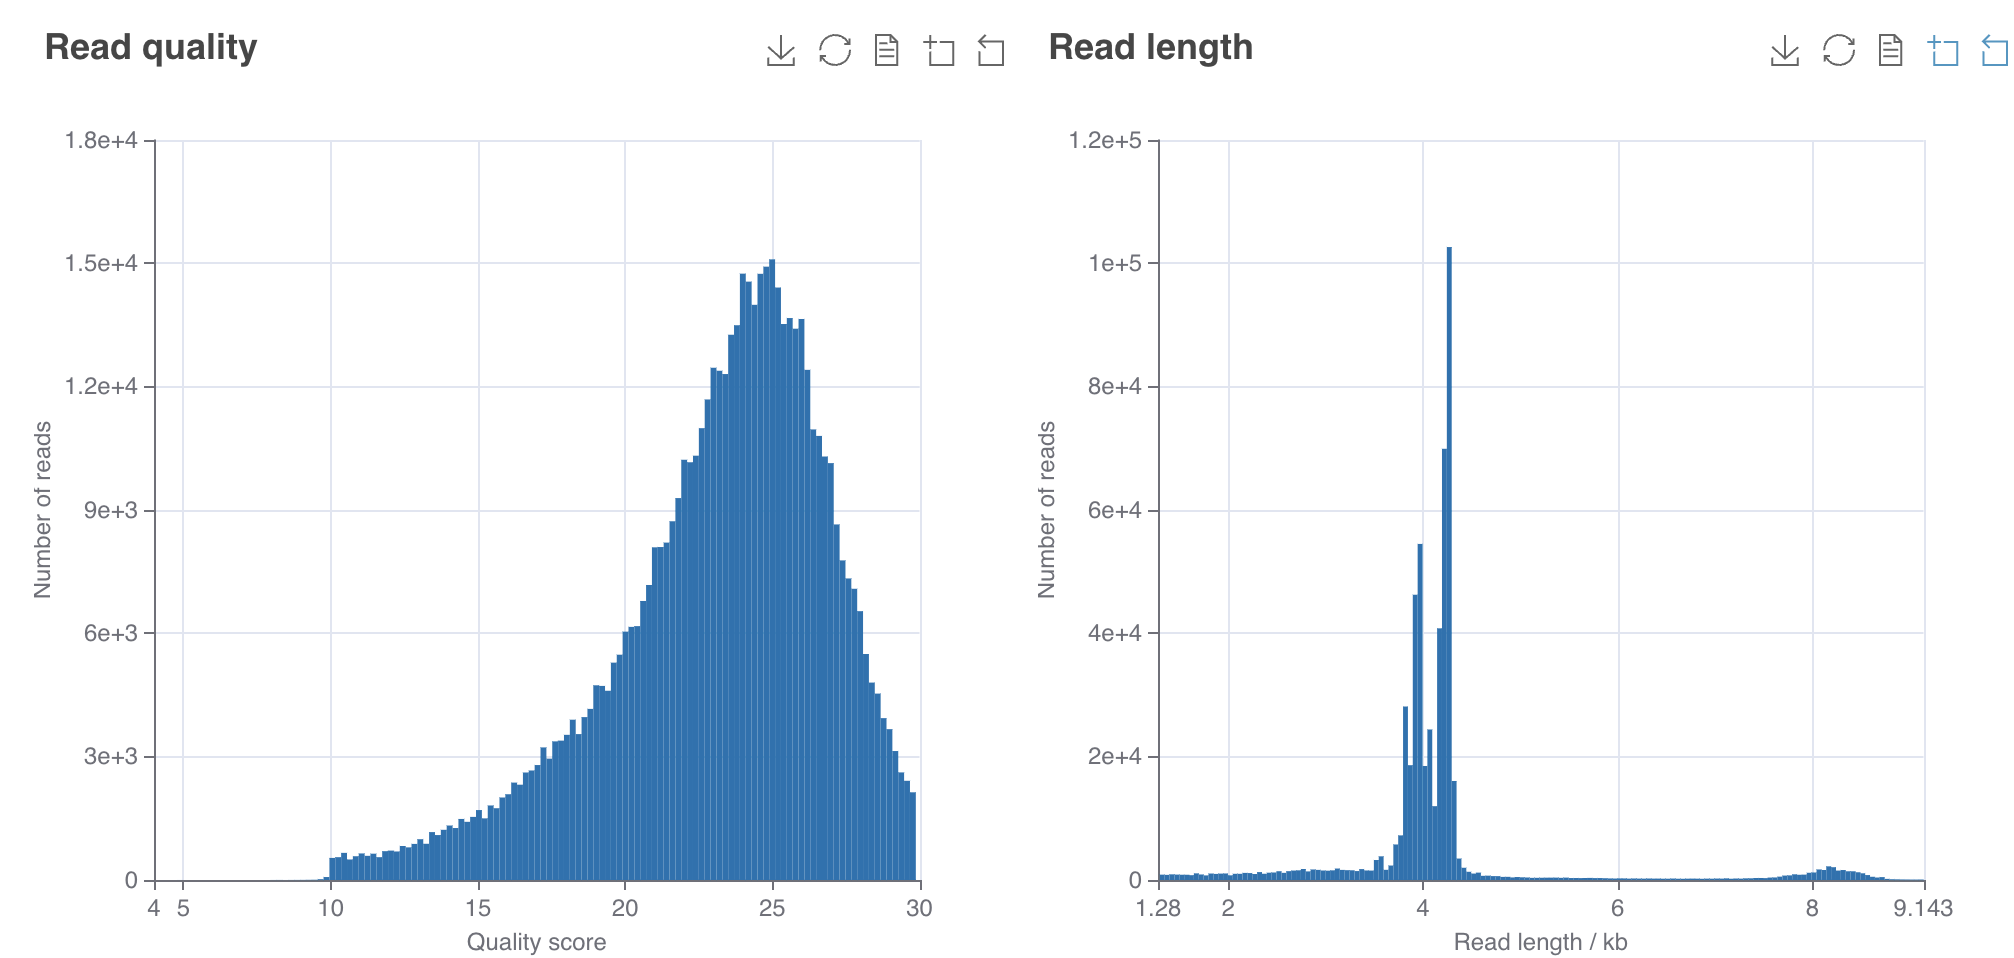
\includegraphics[width=4.16667in,height=\textheight]{./img/basecallsummary.png}
\caption{``Example of quality distribution of 4kb amplicon reads basecalled at super high accuracy with dorado.''}
\end{figure}

\begin{figure}
\centering
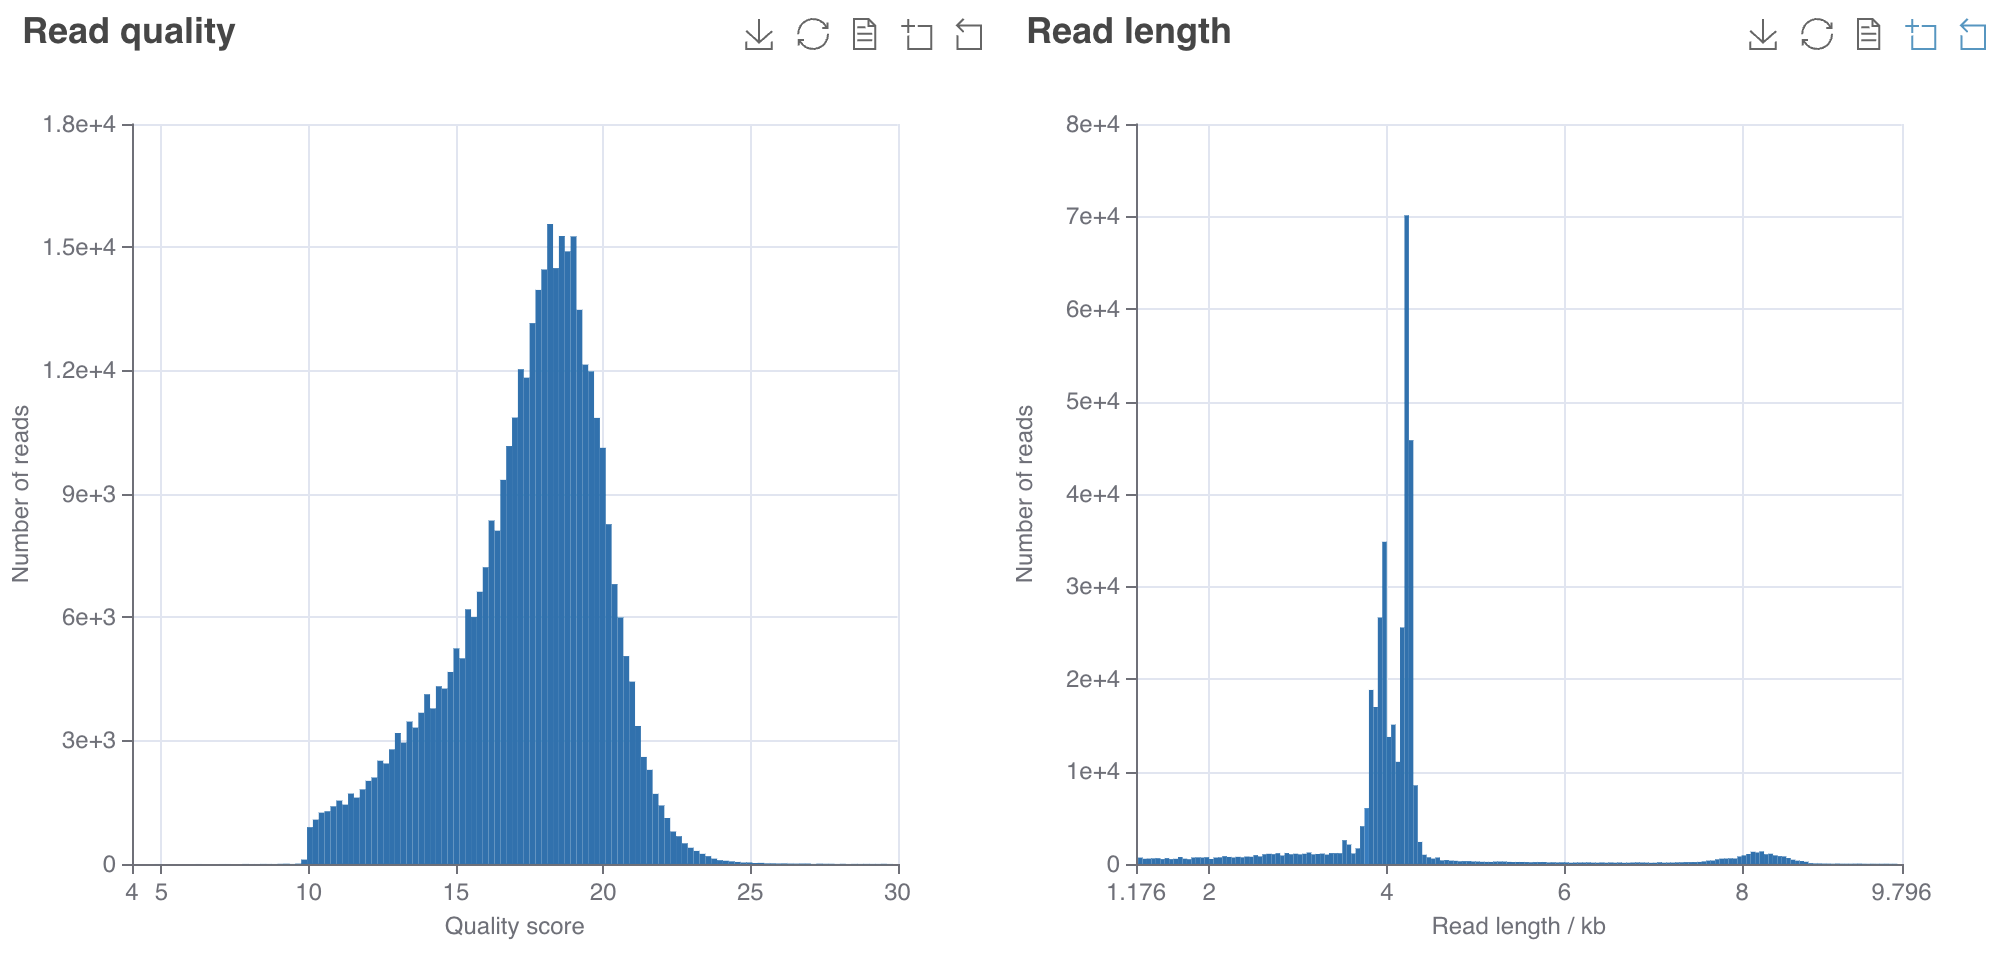
\includegraphics[width=4.16667in,height=\textheight]{./img/basecallsummaryHAC.png}
\caption{``Example of quality distribution of 4kb amplicon reads basecalled at high accuracy with dorado.''}
\end{figure}

\chapter{Protocol}\label{protocol}

\section{DNA extraction}\label{dna-extraction}

\subsection{Checklist}\label{checklist}

\begin{itemize}
\tightlist
\item
  Extraction kit - \href{https://www.qiagen.com/au/resources/resourcedetail?id=9bb59b74-e493-4aeb-b6c1-f660852e8d97&lang=en}{DNeasy Powersoil Pro, Qiagen, Hilden, Germany}. See Section \ref{prerequisites} for more details.
\item
  Alternatively the high throughput version of the kit used with the QIAcube \href{https://rmiteduau-my.sharepoint.com/personal/christian_krohn_rmit_edu_au/Documents/Experiments/2025_ETPSequencingProject/_\%09https:/www.qiagen.com/au/products/discovery-and-translational-research/dna-rna-purification/dna-purification/microbial-dna/dneasy-96-powersoil-pro-qiacube-ht-kit}{DNeasy 96 PowerSoil Pro QIAcube HT Kit}.
\item
  Vortex with 24 x 1.5 mL tube adapter (e.g.~Vortex Genie 2 + adapter). Alternatively, a PowerLyzer Homogenizer.
\item
  NanoDrop spectrophotometer to assess DNA quality.
\item
  Qubit fluorometer to accurately measure DNA concentrations.
\end{itemize}

\subsection{Steps}\label{steps}

\begin{itemize}
\tightlist
\item
  Follow the extraction kit's protocol with 15 mins bead beating using a Vortex-Genie and 24-tube adapter. Reduce this to 10 mins if less than 24 samples are extracted or if shearing of DNA should be minimised.
\item
  Measure DNA quality using DNA extract (1 µL) using a Nanodrop spectrophotometer
\item
  Measure DNA concentration using a Qubit fluorometer.
\item
  Into a 96-well plate, normalise extracted DNA to required PCR concentrations. For example, if 10 ng template is required for PCR, normalise DNA to 5 ng/µL.
\item
  Store DNA at 4˚C until library preparation - no more than 1 week.
\item
  Store DNA at -20˚C if sequencing is more than 1 week away.
\end{itemize}

\section{Amplification of 16S-ITS-23 operon}\label{amplification-of-16s-its-23-operon}

\subsection{Checklist}\label{checklist-1}

\begin{itemize}
\tightlist
\item
  10 mM dNTPs (N0447S, New England Biolab)
\item
  Q5 Hot Start High-Fidelity DNA Polymerase (M0493, New England Biolab)
\item
  10 µM Forward Primer A519F (CAGCMGCCGCGGTAA) \citep{Martijn2019}
\item
  10 µM Reverse Primer U2428R (CCRAMCTGTCTCACGACG) \citep{Martijn2019}
\item
  JetSeq Clean Magnetic beads - or equivalent (MER-BIO-68031, Millenium Science) - to clean up PCR products
\item
  twin.tec® PCR plate 96 LoBind, semi skirted (0030129504, Eppendorf)
\item
  Nuclease-free water
\item
  10 mM Tris-HCl pH 8.0 with 50 mM NaCl (UltraPure™ 1M Tris-HCI, pH 8.0 \#15568025 \& NaCl (5 M), RNase-free \#AM9760G, Thermo Fisher)
\item
  HyperLadder 1kb (BIO-33025, Bioline, Millenium Science)
\item
  80\% ethanol, freshly prepared in nuclease-free water
\item
  Qubit 1X dsDNA BR Assay Kit (Q33266, Thermo Fisher)
\end{itemize}

\textbf{Notes}

\begin{itemize}
\tightlist
\item
  Do not vortex tubes during library preparation to prevent DNA fragmentation. Fragmentation of amplicons may lead to incomplete reads.
\item
  The primer amplifies the whole rrn operon.
\end{itemize}

Benefits of targeting the whole rrn operon:

\begin{itemize}
\tightlist
\item
  Superior species-level resolution and accuracy \citep{Cusco2018, Srinivas2024}.
\item
  Covers Bacteria and Archaea.
\end{itemize}

Risks of targeting the whole rrn operon:

\begin{itemize}
\tightlist
\item
  Not as representative of true abundances as full-length 16S amplicons.
\item
  Species with unlinked 16S and 23S rrn DNA will be missed with this approach (for example \textless{} 9\% of rRNA genes in wastewater sludge \citep{Brewer2020}).
\end{itemize}

\subsection{PCR}\label{pcr}

Time required: \textasciitilde4 hrs incl.~2hrs, 40mins PCR.

\begin{itemize}
\tightlist
\item
  Prepare a PCR mastermix for the required number of 50-µl reactions (Table 3.1). It may be necessary to combine two 50 µl reactions for each sample to produce sufficient amplicon mass for a final concentration of 200 fmol as input for the Native Barcoding Kit from Oxford Nanopore.
\item
  Add 3 µl of eDNA (5ng /µl) into a 96-well plate (e.g.~Eppendorf twin.tec® PCR plate 96 LoBind, semi-skirted) using a multichannel pipette.
\item
  Add 47 µl of mastermix using a multichannel pipette and carefully pipette up and down 10 x
\item
  Run thermocycler (Table 3.2).
\item
  Verify amplification length via 1\% agarose gel electrophoresis @ 100V for 30 min including a 1 kb ladder.
\item
  Store at 4˚C overnight if needed.
\end{itemize}

\textbf{Important}:

\begin{itemize}
\item
  Use hot start polymerase for ease of use, with high fidelity/accuracy and one that is suitable for long amplicons. For example, Q5 High- Fidelity DNA Polymerase kit (New England Biolabs) with GC enhancer \citep{Martijn2019}.
\item
  ≤ 200 fmol is required per sample for the Native Barcoding Kit from ONP. Based on 4.25 kb (4-4.5kb), the final DNA concentration after cleaning up PCR products should be no less than 48 ng/µL (at 11.5 µl input volume) - giving 552 ng of 4.25kb amplicons.
\item
  It may require two PCR reactions to achieve the required DNA amount (200 fmol); e.g.~pool 2 x 50µl PCR products, clean combined and elude in 32.5 µl Tris. Check if 25 cycles (instead of 30) are enough to get sufficient yield. A lower cycle number lowers the risk of errors.

  ~ ~
\end{itemize}

\begin{table}

\caption{\label{tab:table}List of components for each reaction (each tube) for PCR. See https://www.neb.com/en-au/protocols/2012/08/30/pcr-using-q5-hot-start-high-fidelity-dna-polymerase-m0493 for details.  }
\centering
\begin{tabular}[t]{lll}
\toprule
Component & 50 µl reaction & Final concentration\\
\midrule
5X Q5 Reaction Buffer - M0493S NEB & 10 µL & 1X\\
10 mM dNTPs N0447S & 1 µL & 200 µM\\
10 µM Forward Primer & 2.5 µL & 0.5 µM\\
10 µM Reverse Primer & 2.5 µl & 0.5 µM\\
Template DNA - 15 ng & 3 µL (5 ng/µL) & < 1,000 ng\\
\addlinespace
Q5 Hot Start High-Fidelity DNA Polymerase -M0493S NEB & 1.0 µL & 0.04 U/µL\\
5X Q5 High GC Enhancer M0493S NEB & 10 µL & (1X)\\
Nuclease-Free Water & to 50 µL & \\
\bottomrule
\end{tabular}
\end{table}

~

\begin{table}

\caption{\label{tab:table2}Thermocycler conditions (Martijn et al 2019).}
\centering
\begin{tabular}[t]{l}
\toprule
Cycle conditions\\
\midrule
1 cycle:\\
30 s - Initial Denaturation 98 degree C\\
30 cycles:\\
10 s - 98 degree C\\
30 s -  64 degree C\\
\addlinespace
210 s - 72 degree C\\
1 cycle:\\
10 min - Final Extension  72 degree C\\
\bottomrule
\end{tabular}
\end{table}

\hfill\break

\section{PCR product clean-up}\label{pcr-product-clean-up}

Clean with 0.6X JetSeq Clean Magnetic beads (or equivalent) and wash twice with 80\% ethanol. This follows a similar protocol to the Illumina 16S-metagenomics library prep guide in case you are familiar with that.

Time required: \textasciitilde{} 1 hr per 24 samples.

\subsection{Checklist}\label{checklist-2}

\begin{itemize}
\tightlist
\item
  Magnetic rack for 96-well plate (e.g.~\#AM10027 Thermo Fisher)
\item
  80\% ethanol, freshly prepared in nuclease-free water
\item
  Nuclease-free water
\item
  10 mM Tris-HCl pH 8.0 with 50 mM NaCl (UltraPure™ 1M Tris-HCI, pH 8.0 \#15568025 \& NaCl (5 M), RNase-free \#AM9760G, Thermo Fisher)
\item
  JetSeq Clean Magnetic beads (MER-BIO-68031, Millenium Science) or equivalent - to clean up PCR products
\item
  Qubit 1X dsDNA BR or HR Assay Kit (Q33266 or Q33231, Thermo Fisher)
\item
  HyperLadder 1kb (BIO-33025, Bioline, Millenium Science)
\item
  A worksheet to enter concentrations and calculate volumes for normalising DNA to 200 fmol
\end{itemize}

\textbf{Note}

Use wide bore tips for adding mag beads and subsequent (careful) mixing by pipetting to minimise DNA fragmentation.

\subsection{Steps}\label{steps-1}

\begin{itemize}
\tightlist
\item
  Pool replicate reactions into one well - e.g.~2 x 50 µl = 100 µl in one well.
\item
  Using a multi-channel pipette, add 0.6X beads to PCR products in the same wells (e.g.~60 µl to 100 µl pooled reactions), pipette 10 x up and down and/or a gentle vortex after sealing the plate, careful not to spill (Vortex Genie speed 2).
\item
  10 min incubation at RT
\item
  Place plate on a magnetic rack for 5 mins and remove supernatant.
\item
  Wash twice with 200 µl 80\% ethanol in same 96-well plate, discard ethanol and let evaporate for \textasciitilde{} 5 mins or until completely removed.
\item
  Take plate off magnet and elude pellet to a volume that provides appropriate DNA concentrations

  \begin{itemize}
  \tightlist
  \item
    e.g.~add 32.5 µl of elution buffer (10 mM Tris 50mM NaCl). The pellet will be stuck higher than the buffer surface in the well.
  \item
    Hence, pipetting up and down 20--30 x may be necessary to carefully wash the pellet of the tube wall, using a wide bore tip.
  \item
    And/or centrifuge plate at 200 rcf for 1 min.
  \end{itemize}
\item
  Off-magnet, incubate plate for 15 minutes at 37°C (e.g.~in a water bath with only the wells submerged in water). Every 2 minutes, agitate the sample by gently vortexing the plate for 10 seconds (after sealing plate) to encourage DNA elution - and spin plate down.
\item
  Collect 32 µl of cleaned DNA after \textasciitilde{} 5 mins on magnet using wide bore tips.
\item
  Quantify and record amplicon concentrations using Qubit HS or BS chemistry and record values. Based on 4 kb amplicons, the final DNA concentration after cleaning up PCR products should be no less than 45 ng/µL to have sufficient material for downstream library preparation (200 fmol, \textgreater{} 520 ng of 4 kb amplicons).
\item
  Verify amplification length via 0.5-1\% agarose gel electrophoresis @ 100V for 30 min including a 1 kb ladder.
\item
  For each sample calculate volumes required of cleaned DNA and H\textsubscript{2}0 to get 200 fmol in 11.5 µl - for library preparation with the Native Barcoding Kit from Oxford Nanopore. Use V1 = C2*V2 / C1, where V1 = x, C1 = DNA concentrations (ng/µl), C2 = 45.22 ng/µl, V2 = 11.5 µl). H\textsubscript{2}0 volume = 11.5 µl - V1. These volumes will be used in the next step.
\end{itemize}

\hfill\break

\begin{figure}
\centering
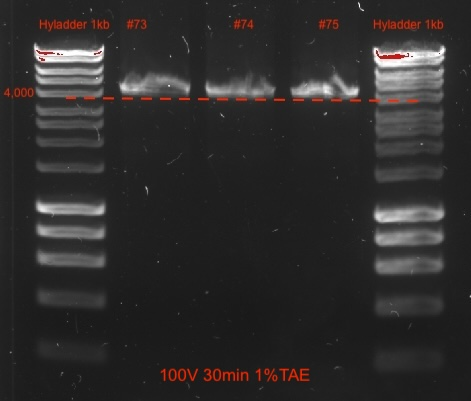
\includegraphics[width=3.125in,height=\textheight]{./img/PCR_gel.jpg}
\caption{Gel confirming amplification of \textasciitilde4 kb amplicons}
\end{figure}

\hfill\break

\begin{figure}
\centering
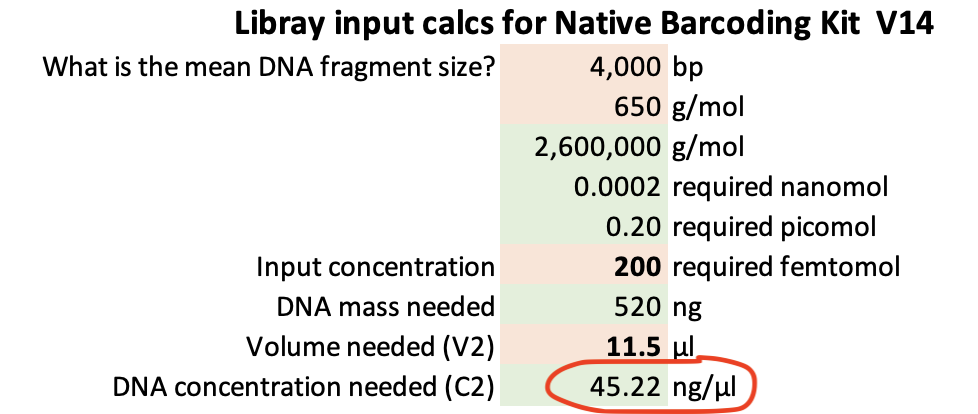
\includegraphics[width=4.16667in,height=\textheight]{./img/PCR_minDNA.png}
\caption{Target concentration of library to normalise to 200 fmol based on a 4 kb amplicon .}
\end{figure}

\hfill\break

\begin{figure}
\centering
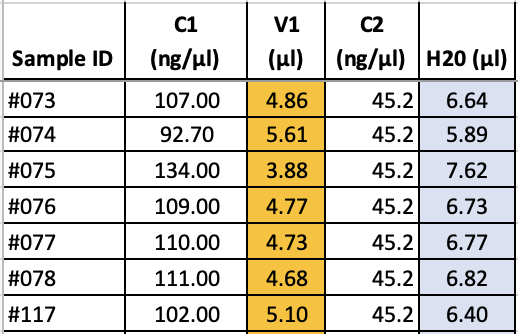
\includegraphics[width=3.125in,height=\textheight]{./img/PCR_C1V1.png}
\caption{Example of a worksheet for calculating volumes (µl) of PCR products and H\textsubscript{2}0 to get 200 fmol in 11.5 µl, required as input for each sample with the Native Barcoding Kit. C1 = DNA concentration (ng/µl), C2 (library concentration) = 45.22 ng/µl, V2 (target volume) = 11.5 µl.}
\end{figure}

~

\section{Library preparation}\label{library-preparation}

DNA Library preparation, including barcoding and pooling of samples (multiplexing). Here the DNA input are \textgreater4 kb amplicons of the 16S-ITS-23S rRNA operon from environmental DNA. The Long Fragment Buffer (LFB) is used (not the Short Fragment Buffer)

Time required: \textasciitilde{} 6 hours from start to finished library ready for loading.

\textbf{Notes}

\begin{itemize}
\tightlist
\item
  Follow the protocol \texttt{Ligation\ sequencing\ amplicons\ -\ Native\ Barcoding\ Kit\ 96\ V14\ (SQK-NBD114.96)-minion.pdf} available on nanoporetech.com. For details about the barcodes check here: \url{https://community.nanoporetech.com/technical_documents/chemistry-technical-document/v/chtd_500_v1_revaq_07jul2016/barcode-sequences}. For final library calculations we assume that around 300 bps are added to the amplicons through barcodes, flanking sequences and adapters. If you know more - let us know on the Github discussion section.
\item
  Update the MinION packages and MinKNOW software.
\item
  Prepare a sample sheet for upload to instrument if desired (not essential but saves a little time when setting up the sequencing in MinKNOW - AND you can use it for demultiplexing with dorado later). More info on how to upload sample sheets \href{https://community.nanoporetech.com/docs/prepare/library_prep_protocols/experiment-companion-minknow/v/mke_1013_v1_revdc_11apr2016/sample-sheet-upload}{here}.
\item
  Amplicon product yields from PCR can vary widely depending on environmental source.
\item
  To achieve consistent, normalised concentrations (200 fmol) across all samples, add appropriate input volume (calculated with C1*V1 = C2*V2) and fill to 11.5 µl with H\textsubscript{2}0 to the first step of the Native Barcoding kit protocol.
\item
  If you plan to sequence after library preparations, insert a flow cell now and do a \textbf{flow cell check} and record the number of pores. This will take around 10 minutes. Afterwards store it at 4˚C until ready to load. We got 1,500-1,750 pores with new flowcells (R10.4.1) that were stored for two weeks at 4 degrees.
\end{itemize}

\subsection{Checklist}\label{checklist-3}

\begin{itemize}
\tightlist
\item
  Native Barcoding Kit (Oxford Nanopore, SQK-NBD114.96)

  \begin{itemize}
  \tightlist
  \item
    End-prep

    \begin{itemize}
    \tightlist
    \item
      DNA Control Sample (DCS)
    \item
      Elution Buffer (EB)
    \end{itemize}
  \item
    Native barcode ligation

    \begin{itemize}
    \tightlist
    \item
      AMPure XP Beads (AXP)
    \item
      EDTA
    \item
      Native Barcodes (NB01-96)
    \end{itemize}
  \item
    Sequencing adapter ligation

    \begin{itemize}
    \tightlist
    \item
      Native Adapter (NA)
    \item
      Elution Buffer (EB)
    \item
      AMPure XP Beads (AXP)
    \item
      Long Fragment Buffer (LFB)
    \end{itemize}
  \end{itemize}
\item
  NEBNext Quick Ligation Module (E6056, New England Biolab)
\item
  NEBNext Ultra II End repair/dA-tailing Module (E7546S, New England Biolab)
\item
  Blunt/TA Ligase Master Mix (M0367, New England Biolab)
\item
  80\% ethanol, freshly prepared in nuclease-free water
\item
  Nuclease-free water
\item
  Qubit 1X dsDNA BR or HR Assay Kit (Q33266 or Q33231, Thermo Fisher)
\item
  Eppendorf LoBind tubes (Eppendorf)
\item
  Magnet for 1.5 ml tubes
\item
  Hula mixer (\#15920D, Thermo Fisher) or similar overhead mixers
\end{itemize}

\subsection{Steps}\label{steps-2}

\textbf{Follow the Nanopore protocol. There are four parts:}

\begin{enumerate}
\def\labelenumi{\arabic{enumi}.}
\item
  End-prepping of 11.5 µL DNA (200 fmol).\\
  Pipetting into the 96-well plate may take time as there are two rounds of pipetting, one for the DNA amplicon volumes and one for H\textsubscript{2}0 volumes to get 200 fmol amplicon DNA in 11.5 µl, as well as the remaining reagents for end-prepping the DNA. It is not possible to use multichannel pipettes for this step.
\item
  Native barcode ligation using 0.75 µL of end-prepped DNA using one of 96 barcodes from the kit for each sample, plus pooling of all barcoded samples into a LoBind tube (1.5 mL).
\item
  Bead clean-up of pooled end-prepped DNA library and elution of 35 µL volume; quantification with Qubit 1X dsDNA HS Assay Kit. We used all of the available end-prepped volume (e.g.~33 µl after Qubit quantification) for the next step, i.o. only 30 µl as per protocol.

  SAFE STOP: Store at 4 ˚C overnight if needed.
\item
  Adapter ligation. Once this step is completed, you get a final volume of 15 µl of clean end-prepped/barcoded/adapter ligated DNA.

  \begin{itemize}
  \item
    We have stored the library at 4˚C overnight and sucessfully sequenced it the next day (although it is preferred to sequence right after adapter ligation).
  \item
    The concentration we achieved was \textasciitilde20-25 ng/µl, which means there was sufficient DNA for two runs. After quantify DNA concentrations with 1 µl DNA there are 14 µl left.
  \item
    Nanopore's recommended loading concentrations are 35--50 fmol at 12 µL volume. For example, at a concentration of 25.3 ng/µl (4,300 kb amplicon) a total of 5.50 µl of DNA library (plus 6.50 µl H\textsubscript{2}0) are sufficient. The remaining 6.50 µl DNA library can be stored in fridge overnight if required.
  \end{itemize}
\end{enumerate}

\begin{figure}
\centering
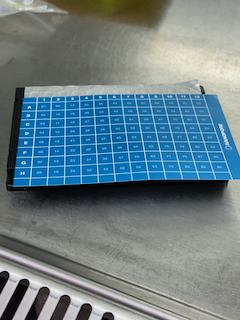
\includegraphics[width=3.125in,height=\textheight]{./img/barcode_ligation.png}
\caption{The Native Barcode Kit (SQK-NBD114.96) comes with 96 individual barcodes}
\end{figure}

\hfill\break

\begin{figure}
\centering
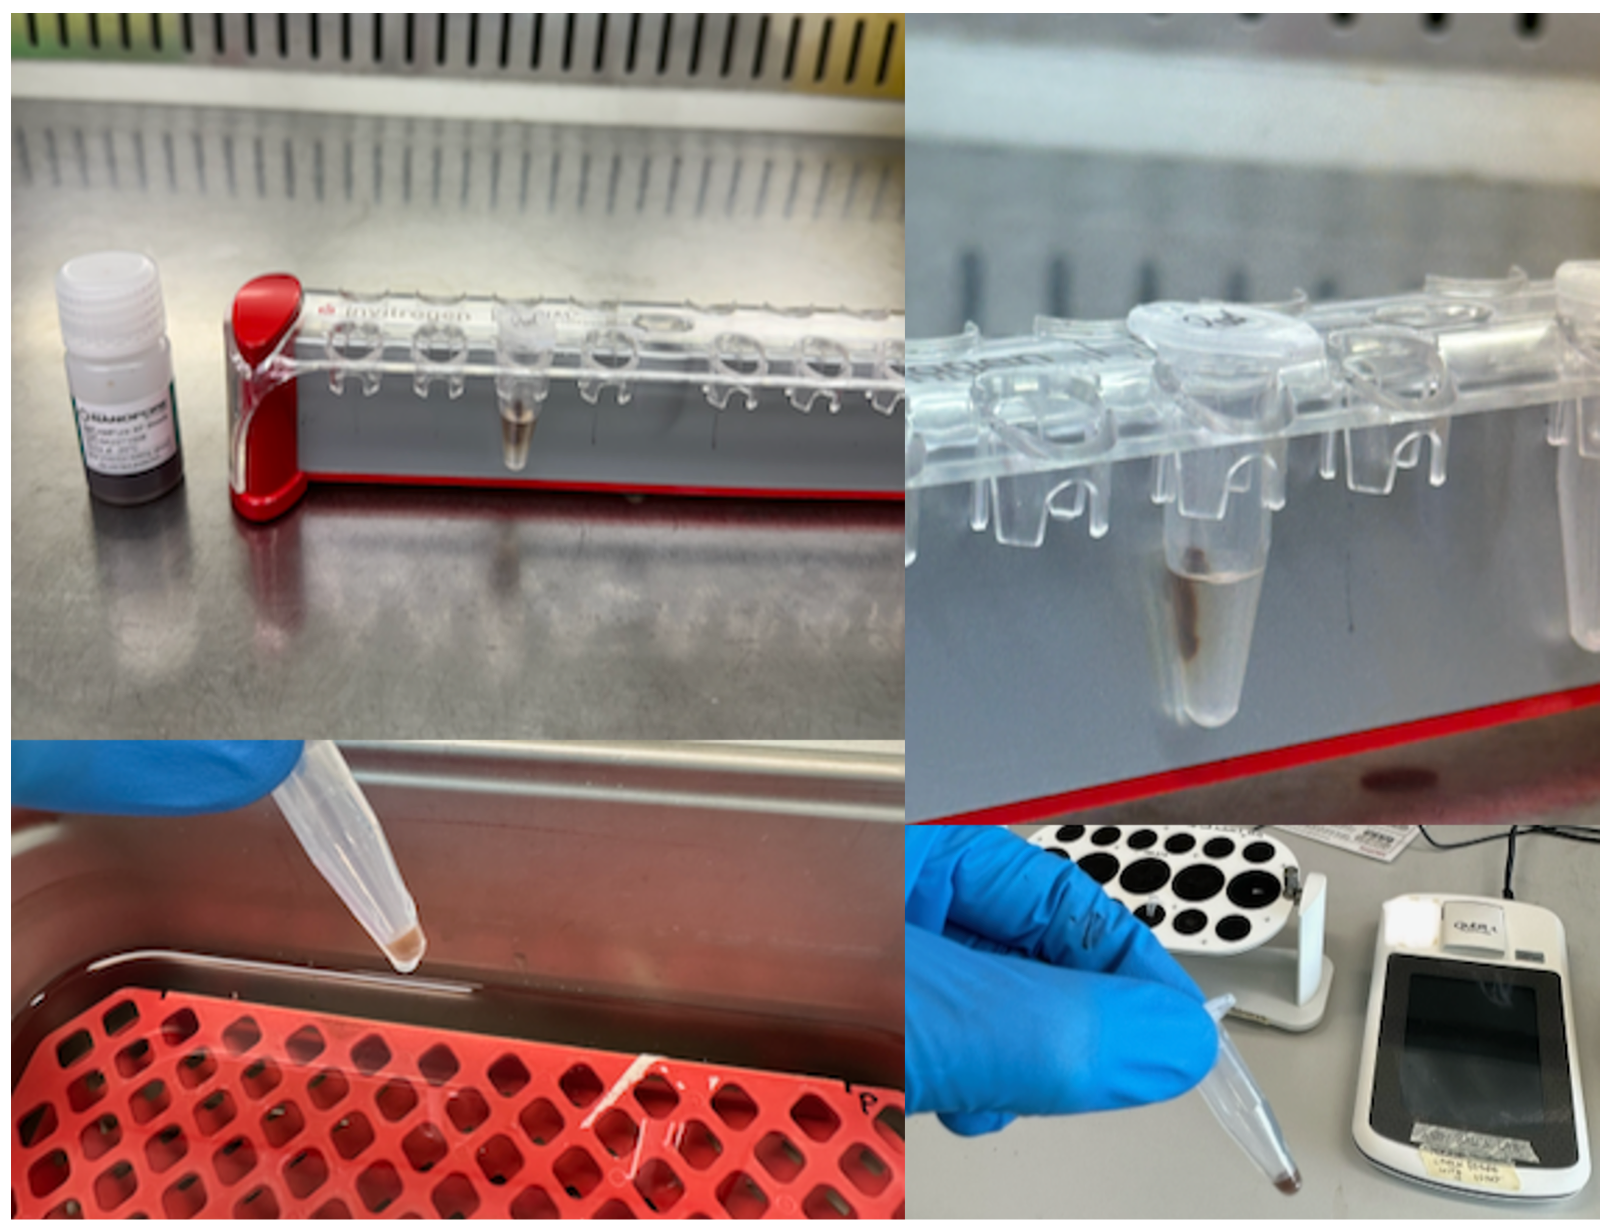
\includegraphics[width=5.20833in,height=\textheight]{./img/libraryprepcleanup_comb.png}
\caption{Bead clean-up of pooled end-prepped and adapter-ligated DNA library}
\end{figure}

\hfill\break

\begin{figure}
\centering
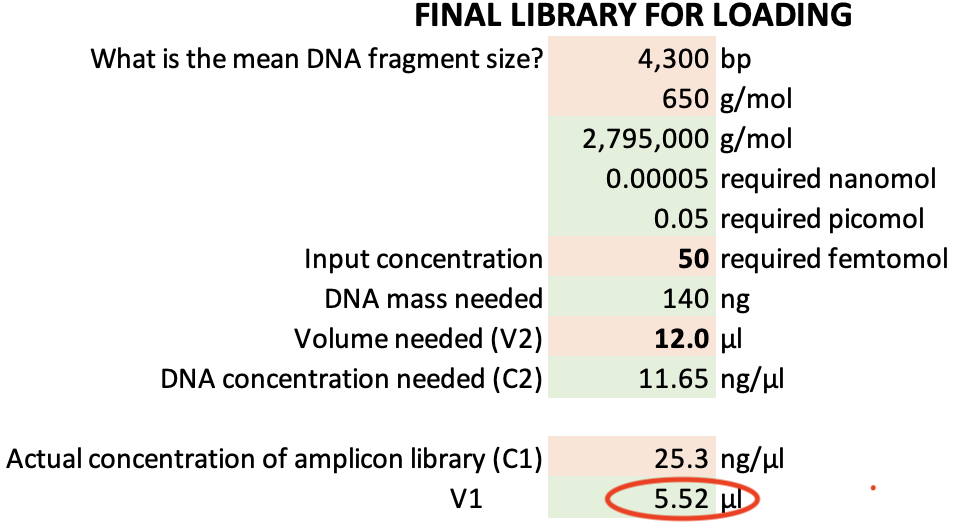
\includegraphics[width=3.125in,height=\textheight]{./img/libraryprepsminDNA.png}
\caption{Calculation to get library volume for loading (In this example we used 5.52 µl of library, plus 6.48µl H20 for a final library volume of 12 µl at 50 fmol concentration)}
\end{figure}

\section{Priming and loading of flow cell - run start}\label{priming-and-loading-of-flow-cell---run-start}

Time required: \textasciitilde10-15 mins for priming and loading. 24 hours for sequencing.

\subsection{Checklist}\label{checklist-4}

\begin{itemize}
\tightlist
\item
  The same protocol: \texttt{Ligation\ sequencing\ amplicons\ -\ Native\ Barcoding\ Kit\ 96\ V14\ (SQK-NBD114.96)-minion.pdf} available on nanoporetech.com
\item
  Bovine Serum Albumin (BSA) (50 mg/ml) (AM2616, InvitrogenTM UltraPure)
\item
  Native Barcoding Kit (Oxford Nanopore, SQK-NBD114.96)

  \begin{itemize}
  \tightlist
  \item
    Flow Cell Flush (FCF)
  \item
    Flow Cell Tether (FCT)
  \item
    Sequencing Buffer (SB)
  \item
    Library Beads (LIB)
  \end{itemize}
\item
  R10.4.1 flowcell (Oxford Nanopore, FLO-MIN114)
\end{itemize}

\subsection{Steps}\label{steps-3}

\textbf{Follow the Nanopore protocol. There are five steps:}

\begin{enumerate}
\def\labelenumi{\arabic{enumi}.}
\tightlist
\item
  Preparation and loading of sequencing buffer and wait for 5 minutes.
\item
  Preparation of library. Nanopore's protocol recommends loading 35--50 fmol at 12 µL volume.
\item
  Loading of remaining sequencing buffer
\item
  Loading of library
\item
  Setting up the run for 24 hours and press start! More details will follow about recommended hours and expected yield based on 24 samples.
\end{enumerate}

\section{Flow cell wash}\label{flow-cell-wash}

Time required: \textasciitilde{} 1.5 hours.

Wash the flow cell once the run has finished. Note that after the wash you can either load a new library directly afterwards or add storage buffer to load a new library later (always store flow at 4 ˚C).

However, it is only possible to check the number of pores (and estimate potential yield) after adding storage buffer. The washing buffer is not suitable for a running a flow cell check. So loading a new library directly is only sensible if the user knows how many active pores to expect. Although, the instrument will do a pore scan at the start, it will be too late once you loaded the new library.

As a gauge, we ran a flowcell with 1,500 pores for 24 hours (loaded with 24 barcoded samples of 16S-ITS-23S amplicons). At the end 558 active pores remained before the wash.

Note that washing the flowcell does not interfer with any active basecalling processes on the Mk1C, which may take days to finish if High Accuracy was chosen.

\subsection{Checklist}\label{checklist-5}

\begin{itemize}
\tightlist
\item
  Flow Cell Wash Kit (e.g.~EXP-WSH004, Oxford Nanopore)
\item
  Protocol \texttt{Flow\ Cell\ Wash\ Kit\ (EXP-WSH004\ or\ EXP-WSH004-XL)-minion.pdf} available on nanopore.com
\end{itemize}

\subsection{Steps}\label{steps-4}

\textbf{Follow the Nanopore protocol. There are three steps:}

\begin{enumerate}
\def\labelenumi{\arabic{enumi}.}
\tightlist
\item
  Preparation of 400 µl washing buffer
\item
  Load 200 µl of washing buffer, wait 5 minutes, then add the remaining 200 µl and wait 1 hour.
\item
  If you plan to store the flowcell for later use - add storage buffer. Otherwise load new library.
\end{enumerate}

\section{Basecalling}\label{basecalling}

Time required: \textasciitilde{} several days depending on computational resources.\\

If you have a PromethION integrated (P2i) you can run Super High Accuracy (SUP) basecalling on the device in almost real time (it has an Nvidia GPU). In that case there is no need to copy POD5 files from the instrument to another computer for SUP basecalling on a separate GPU device.

The below assumes that the \texttt{SQK-NBD114-96} kit was used for preparing the amplicon library.

\subsection{Checklist}\label{checklist-6}

\begin{itemize}
\tightlist
\item
  \href{https://github.com/nanoporetech/dorado}{dorado} installed on an instance or device with either Apple silicon (M1/M2) or Nvidia GPUs (the latest Nvidia RTX 4090 performs best it seems).
\item
  POD5 files from Nanopore sequencer (either copy on USB or connect do instrument folders through \texttt{ssh})
\item
  samplesheet.csv (More details about the sample sheet in the library prep section).
\end{itemize}

\subsection{Steps}\label{steps-5}

\begin{enumerate}
\def\labelenumi{\arabic{enumi}.}
\tightlist
\item
  First let Nanopore sequencer finish basecalling with the Fast model (Unless you have a Promethion Pi, which will provide you with SUP-basecalled bam/fastq files; the following steps are not required in this case).
\item
  Copy POD5 files from sequencer to a GPU-powered computer or instance, into a folder called \texttt{pod5/}. In our case that was 85GB of data (But expect a bit more; our MinION had a power outage just before all pod5 finished generating\ldots{} :( ).
\item
  Run \texttt{dorado\ basecaller\ sup\ pod5/\ \textgreater{}\ calls.bam}.
\item
  Demultiplex the resulting \texttt{.bam} file using \texttt{dorado\ demux\ -\/-kit-name\ SQK-NBD114-96\ -\/-sample-sheet\ samplesheet.csv\ -\/-output-dir\ 16SITS23S\_samples/\ -\/-emit-fastq\ call}.
\end{enumerate}

At the end you should have one \texttt{.fastq} file for each sample, ready for further quality trimming and read classification.

\section{Read classification}\label{read-classification}

The following method (using the \texttt{wf-metagenome} workflow from EPI2ME, with kmer-based read predictions) will provide classified reads of Bacteria and Archaea but, depending on the read quality, will result in some false positives. And abundances will not be a true representation of abundances as no clustering, dereplication or ASV generation is involved. Results will not be comparable to other studies.

However, it will provide read classification to species-level to some degree of certainty, which may be useful in cases when you are not interested in the true representation of relative abundances. For example, if you are after temporal variation or differences between your samples in your experiment.

As rrna operon sequencing is relatively new, the classification methods and databases are still evolving. If you want to explore other methods, I recommend starting with the following papers: \citep{Curry2022}, \citep{Rodriguez-Perez2021} and \citep{mbs:/content/journal/mgen/10.1099/mgen.0.001255}.

\subsection{Checklist}\label{checklist-7}

\begin{itemize}
\tightlist
\item
  \href{https://labs.epi2me.io/}{EPI2ME} installed (we use the desktop version). It requires Docker and Java so if this is your first time installing/using EPI2ME it may take you some time to get started.
\item
  Fastq files in a folder
\item
  \href{https://github.com/wdecoster/chopper}{Chopper} installed.
\end{itemize}

\subsection{Steps}\label{steps-6}

\begin{enumerate}
\def\labelenumi{\arabic{enumi}.}
\tightlist
\item
  Trim fastq files. In this case we used the tool \texttt{Chopper}.
\end{enumerate}

\begin{Shaded}
\begin{Highlighting}[]
\CommentTok{\#!/bin/bash}
\ControlFlowTok{for}\NormalTok{ file }\ControlFlowTok{in} \SpecialCharTok{*}\NormalTok{.fastq; do}
        \CommentTok{\# Construct the output filename based on input filename}
\NormalTok{        output\_file}\OtherTok{=}\StringTok{"$\{file\%.fastq\}\_filtered.fastq"}
        
        \CommentTok{\# Run the chopper command on the current file}
\NormalTok{        chopper }\SpecialCharTok{{-}}\NormalTok{q }\DecValTok{20}  \SpecialCharTok{{-}{-}}\NormalTok{minlength }\DecValTok{3000} \SpecialCharTok{{-}{-}}\NormalTok{maxlength }\DecValTok{5000} \SpecialCharTok{{-}}\NormalTok{i }\StringTok{"$file"} \SpecialCharTok{\textgreater{}} \StringTok{"./Test/$output\_file"}
        
\NormalTok{        echo }\StringTok{"Filtered reads from $file saved to $output\_file"}
\NormalTok{done}
\end{Highlighting}
\end{Shaded}

\begin{enumerate}
\def\labelenumi{\arabic{enumi}.}
\setcounter{enumi}{1}
\tightlist
\item
  Download and select the \texttt{wf-metagenome\ workflow}.\\
  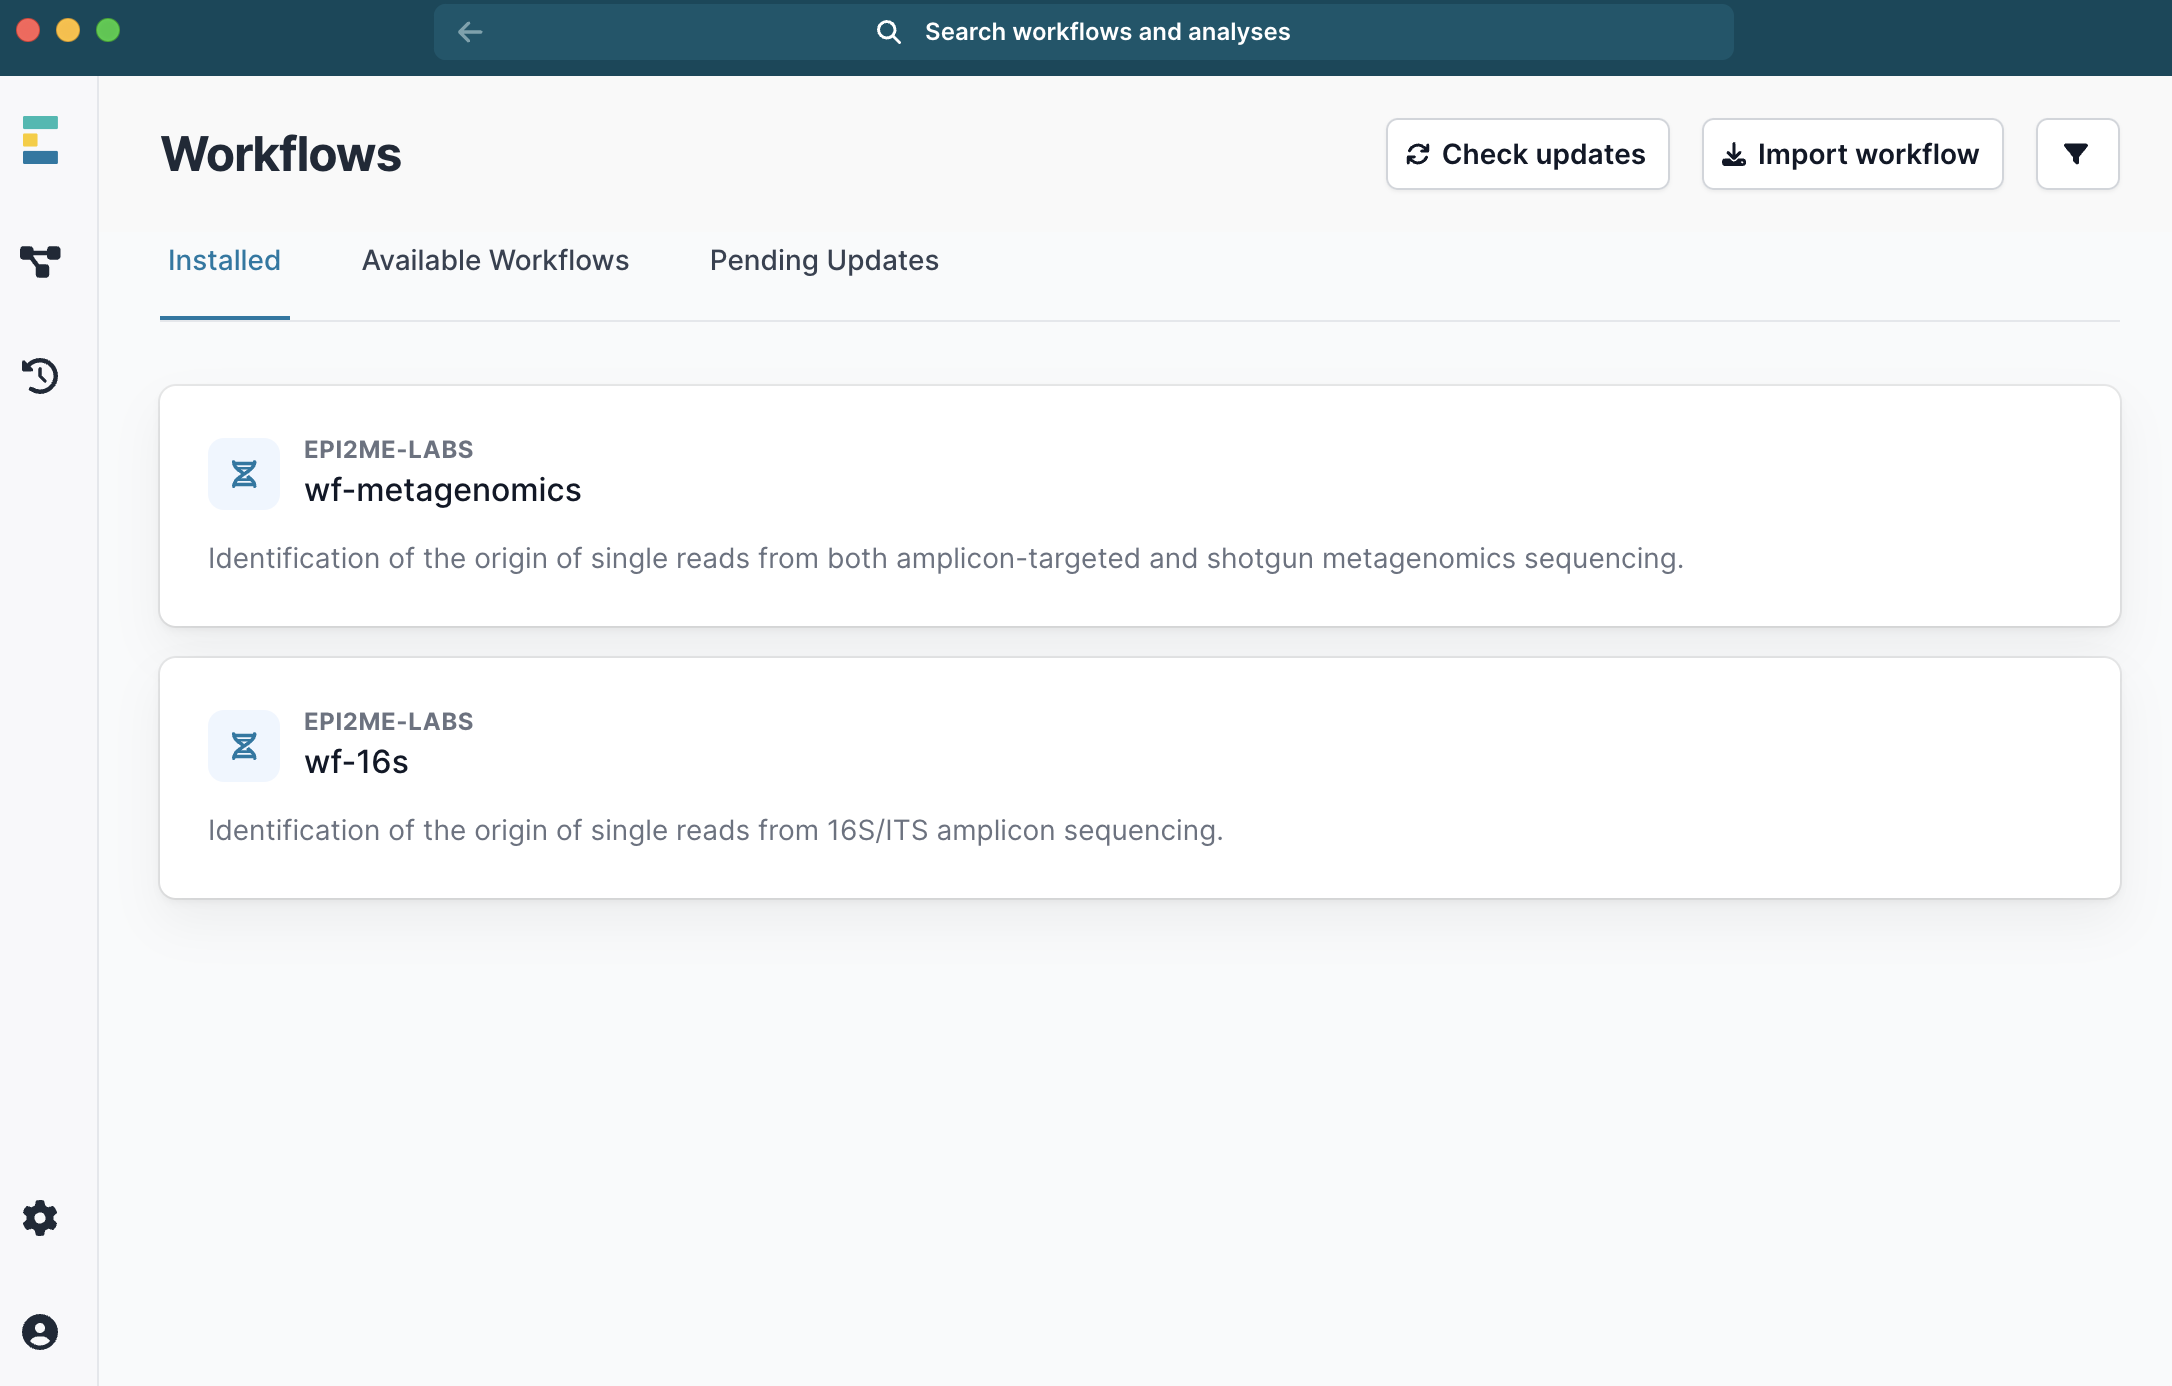
\includegraphics[width=5.20833in,height=\textheight]{./img/wf-metagenome.png}
\item
  Click \texttt{Run\ this\ workflow}, then \texttt{Run\ on\ your\ computer}.
\item
  Select the path your your fastq files.
\item
  Select Classification method. Either kraken2 or minimap2
\item
  Under Reference Options select a database. We used \texttt{ncbi\_16s\_18s\_28s\_ITS}.\\
  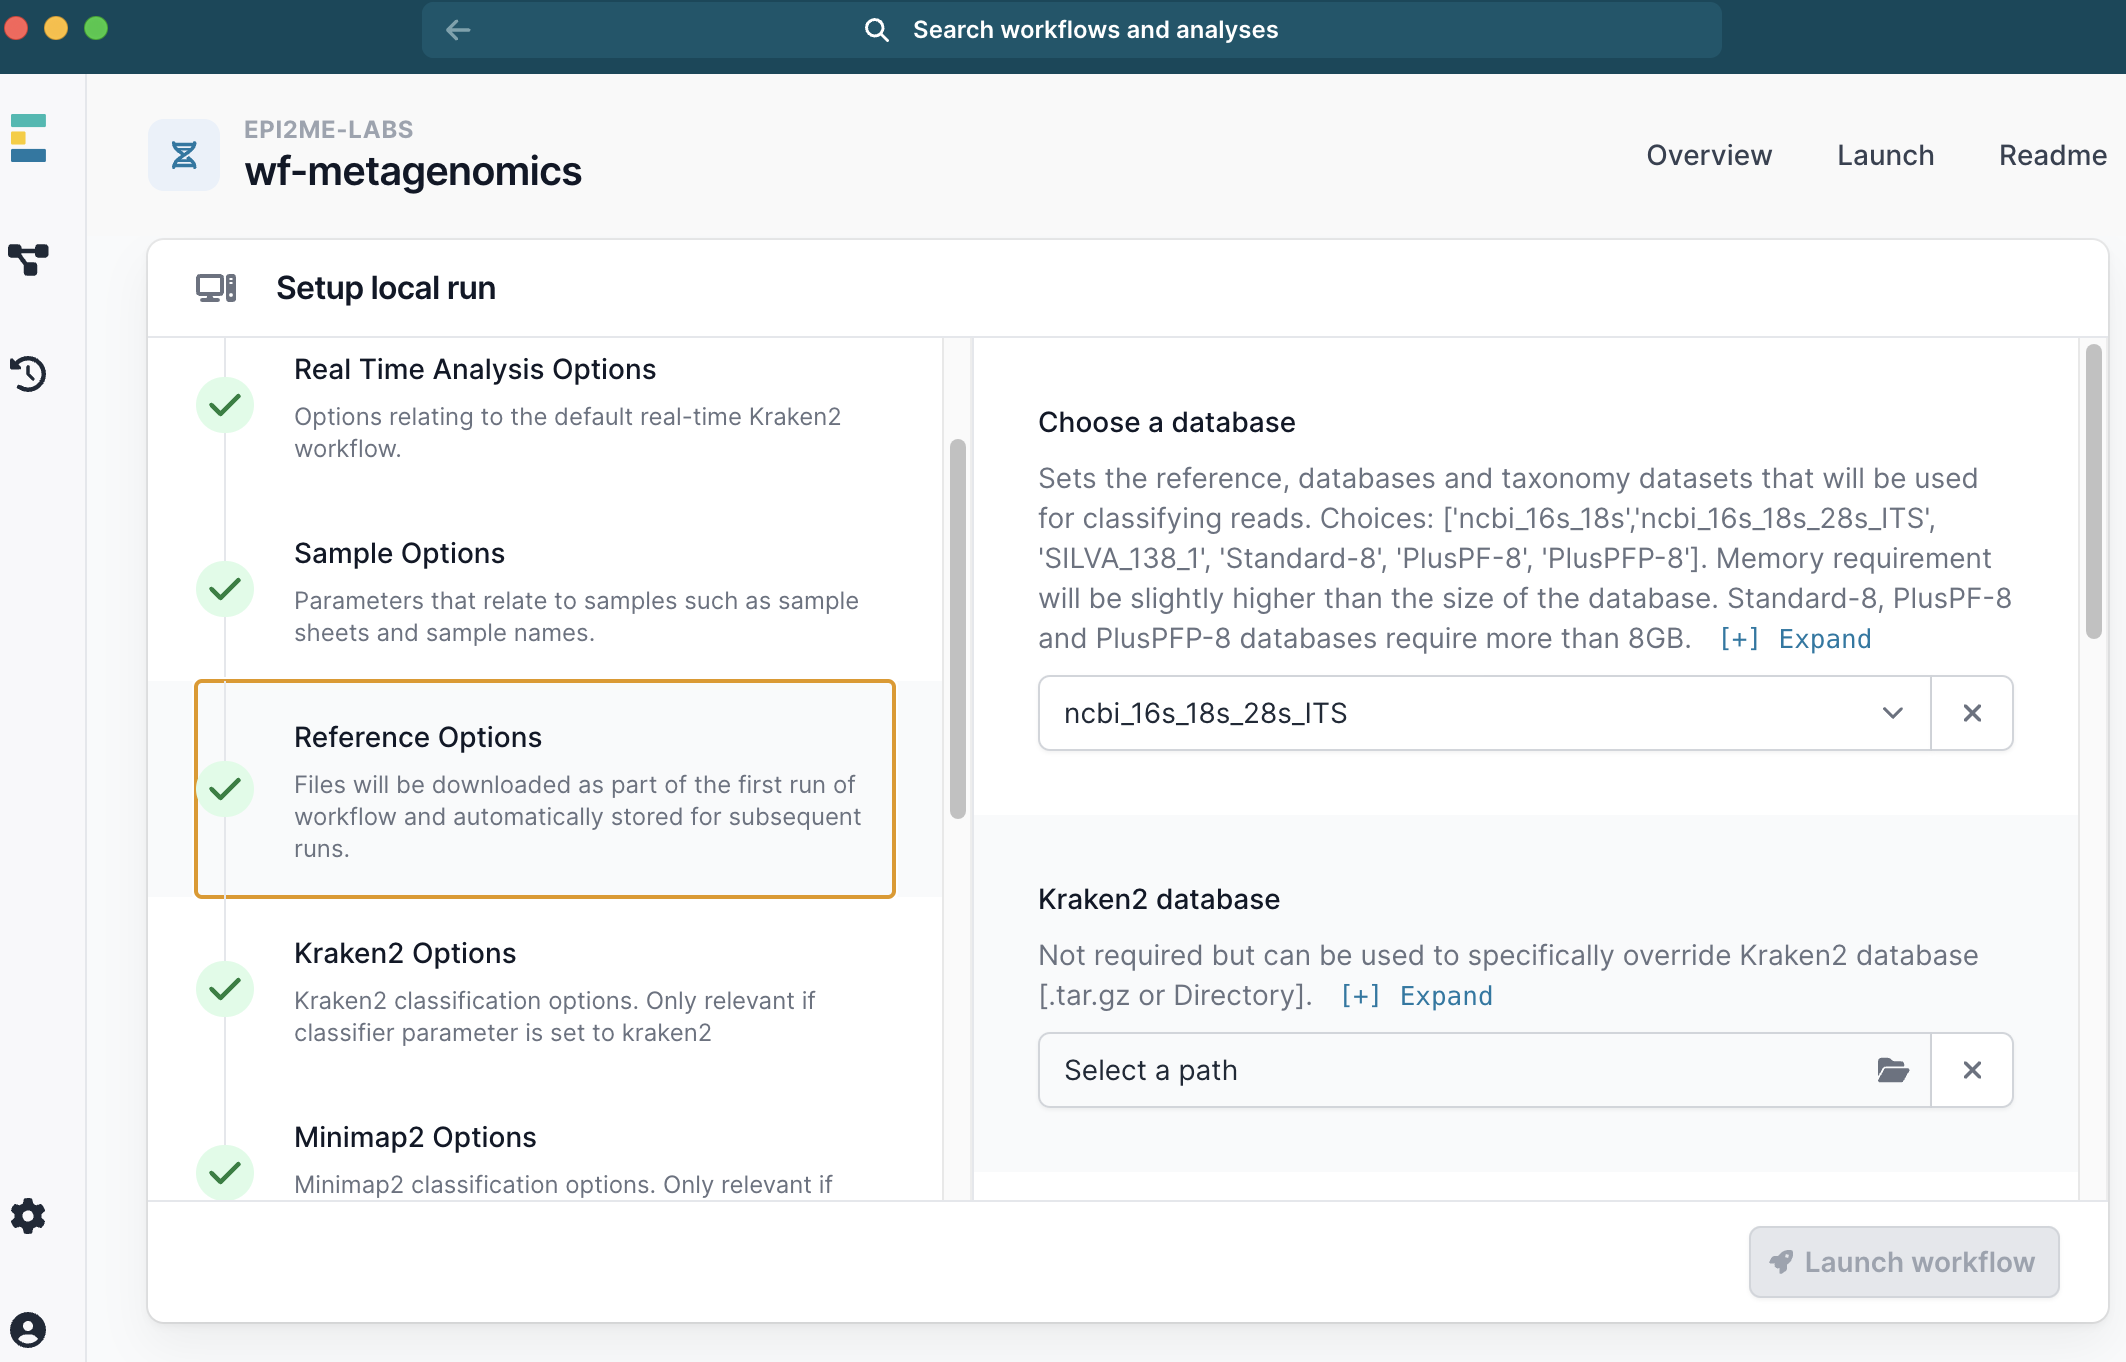
\includegraphics[width=5.20833in,height=\textheight]{./img/database_option.png}
\item
  Under Sample Options select you sample\_sheet.csv. We used \texttt{ncbi\_16s\_18s\_28s\_ITS}.\\
  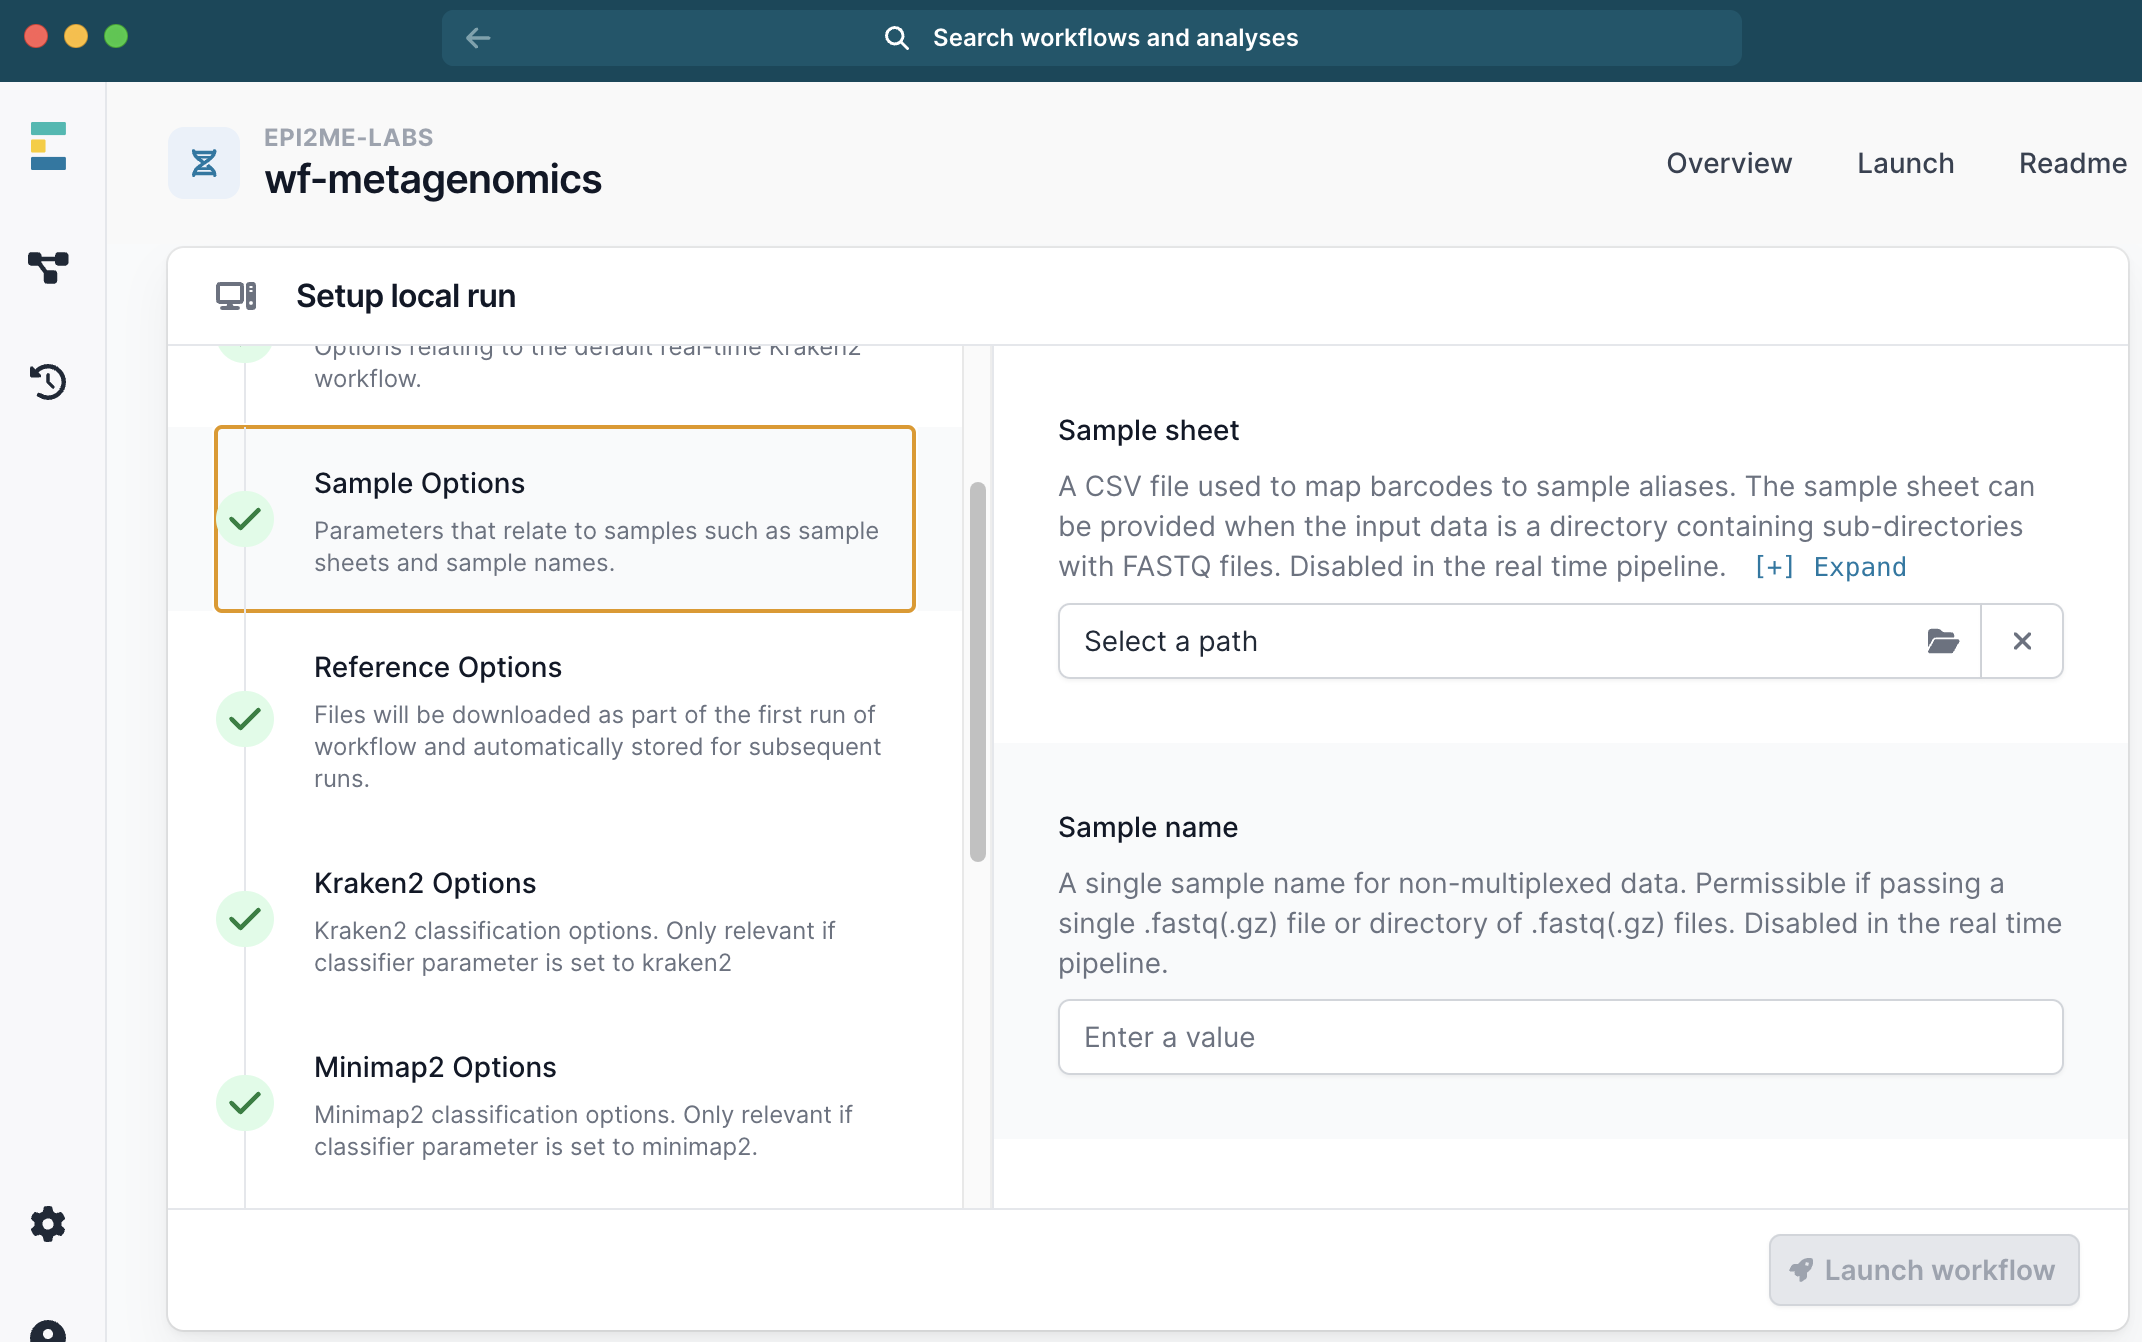
\includegraphics[width=5.20833in,height=\textheight]{./img/samplesheet.png}\\
  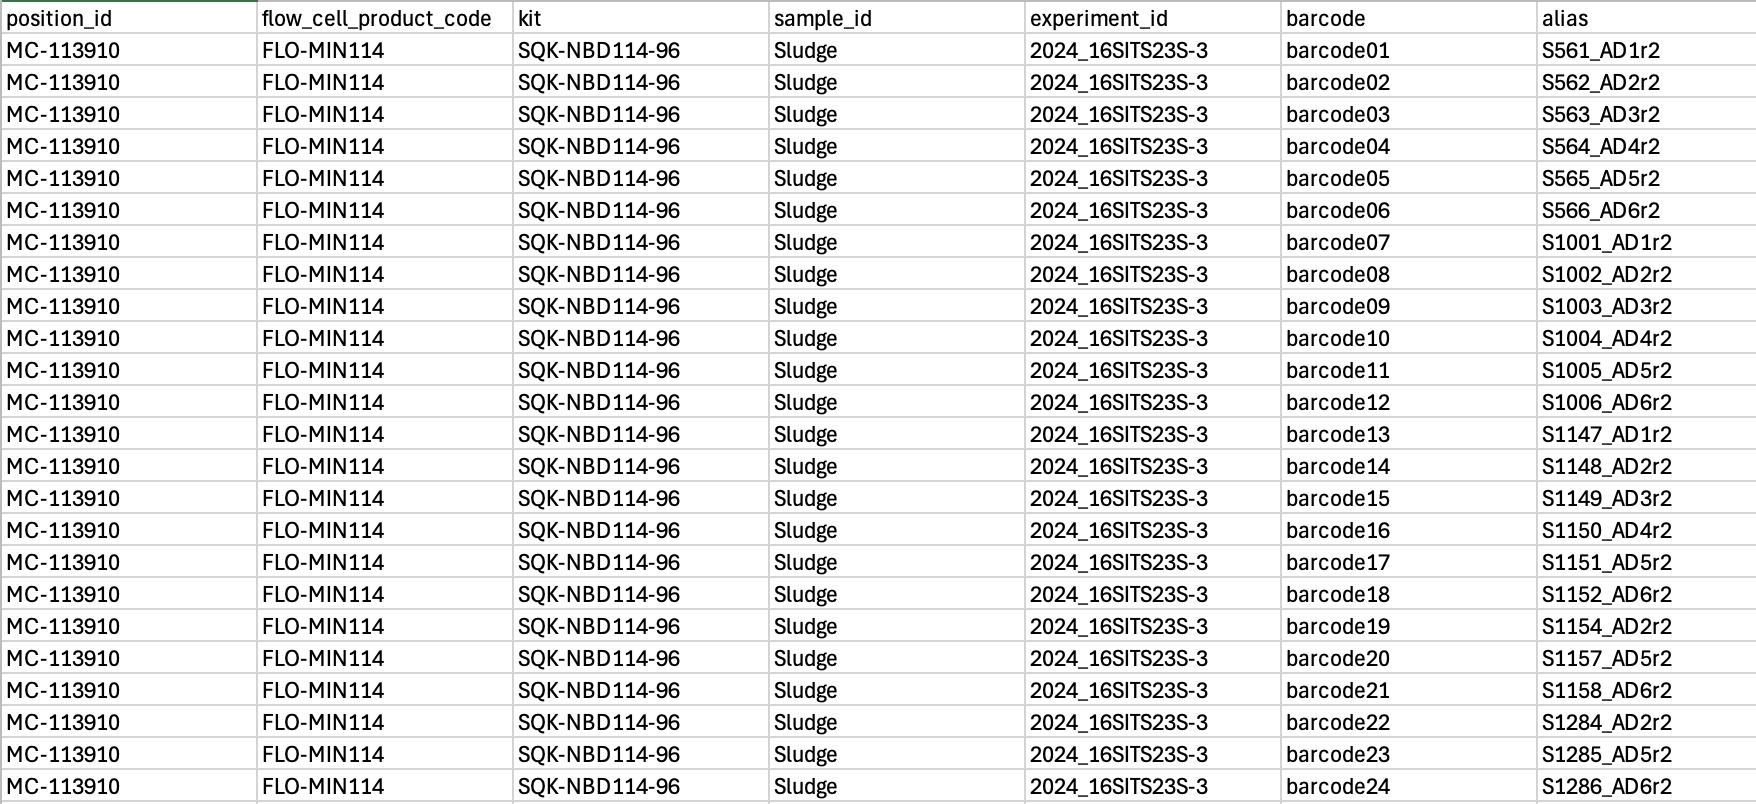
\includegraphics[width=5.20833in,height=\textheight]{./img/sample_sheetxmpl.png}
\item
  Then launch the workflow.
\item
  Once completed your will received \texttt{report.html} with some results, plus a \texttt{.tsv} table with abundances on species-level.
\end{enumerate}

\section{Results}\label{results}

In our case we got \textasciitilde{} 25,000 reads per sample containing 2,137 species. Upon first inspection it is clear that read-depths is too low and that longer sequencing time is required per flowcell than 24 hours for 24 samples. We aim for around 100,000 reads per sample. On a MinION flowcell I would aim to sequence for the full 72 hours next time.

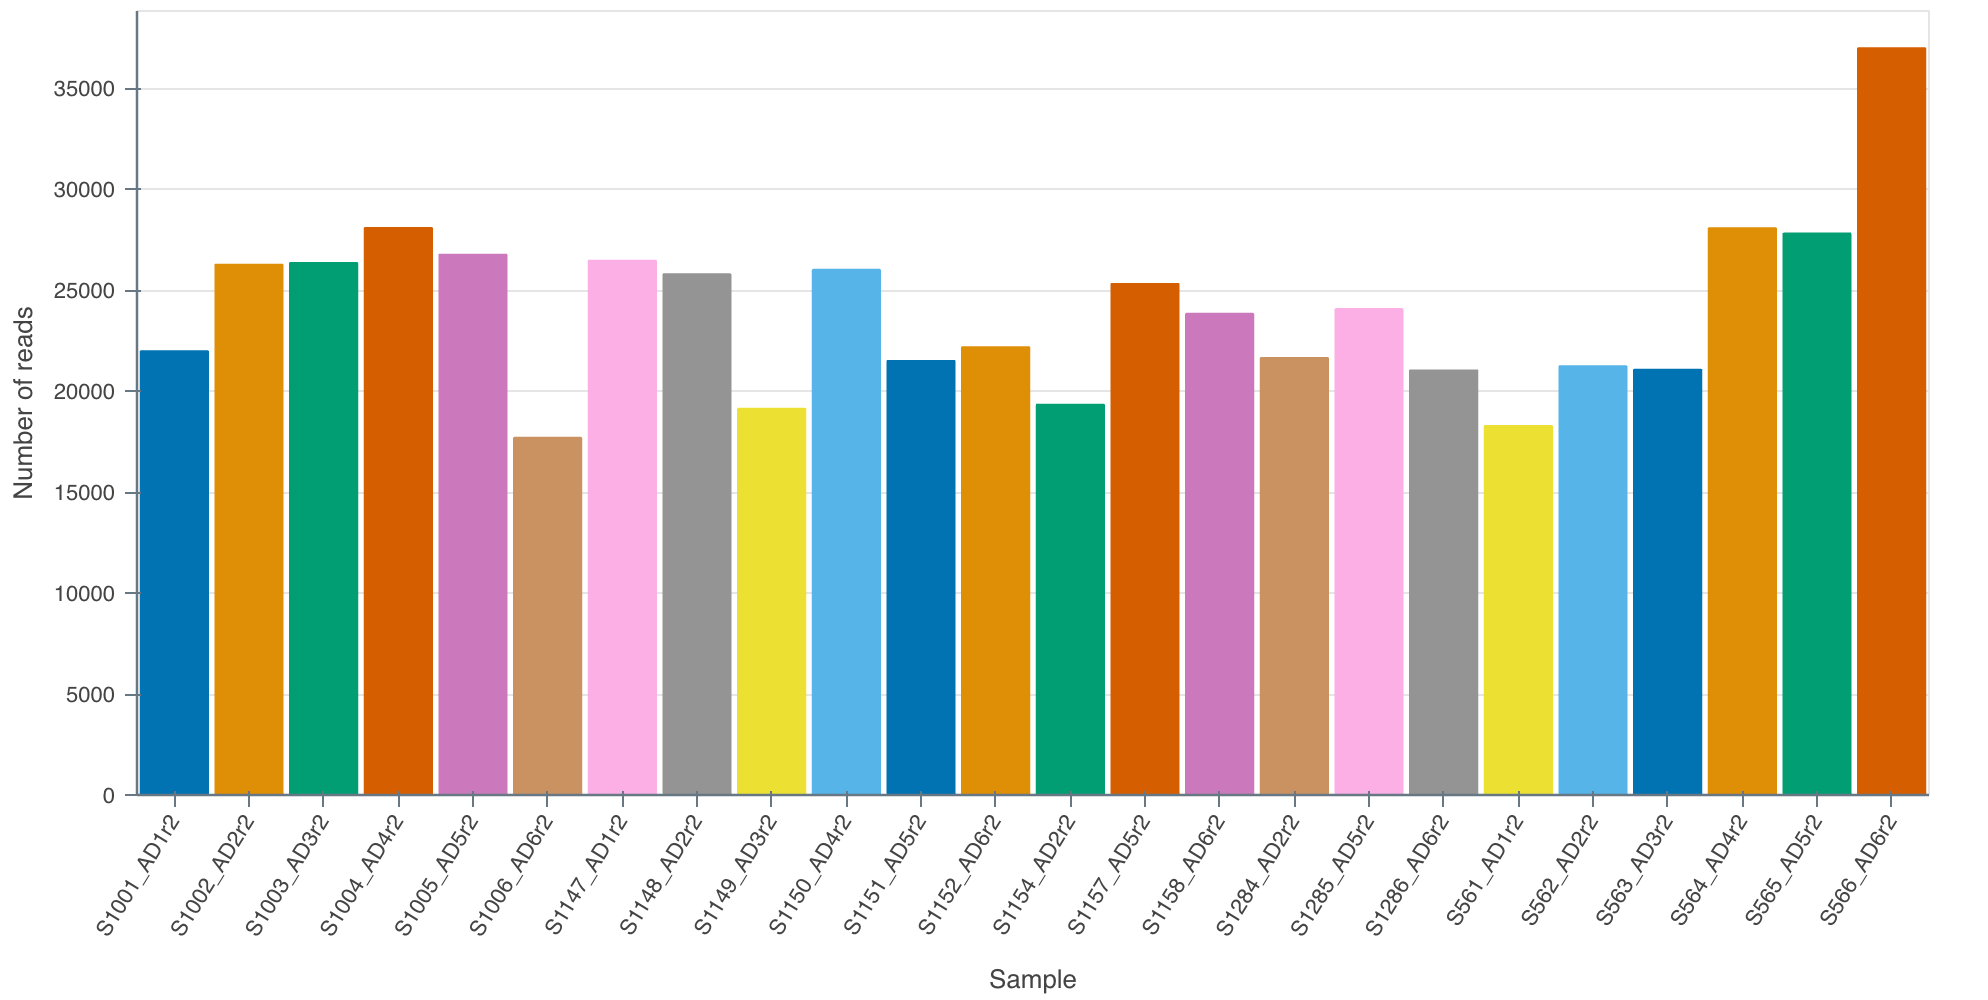
\includegraphics[width=5.20833in,height=\textheight]{./img/results.png}\\
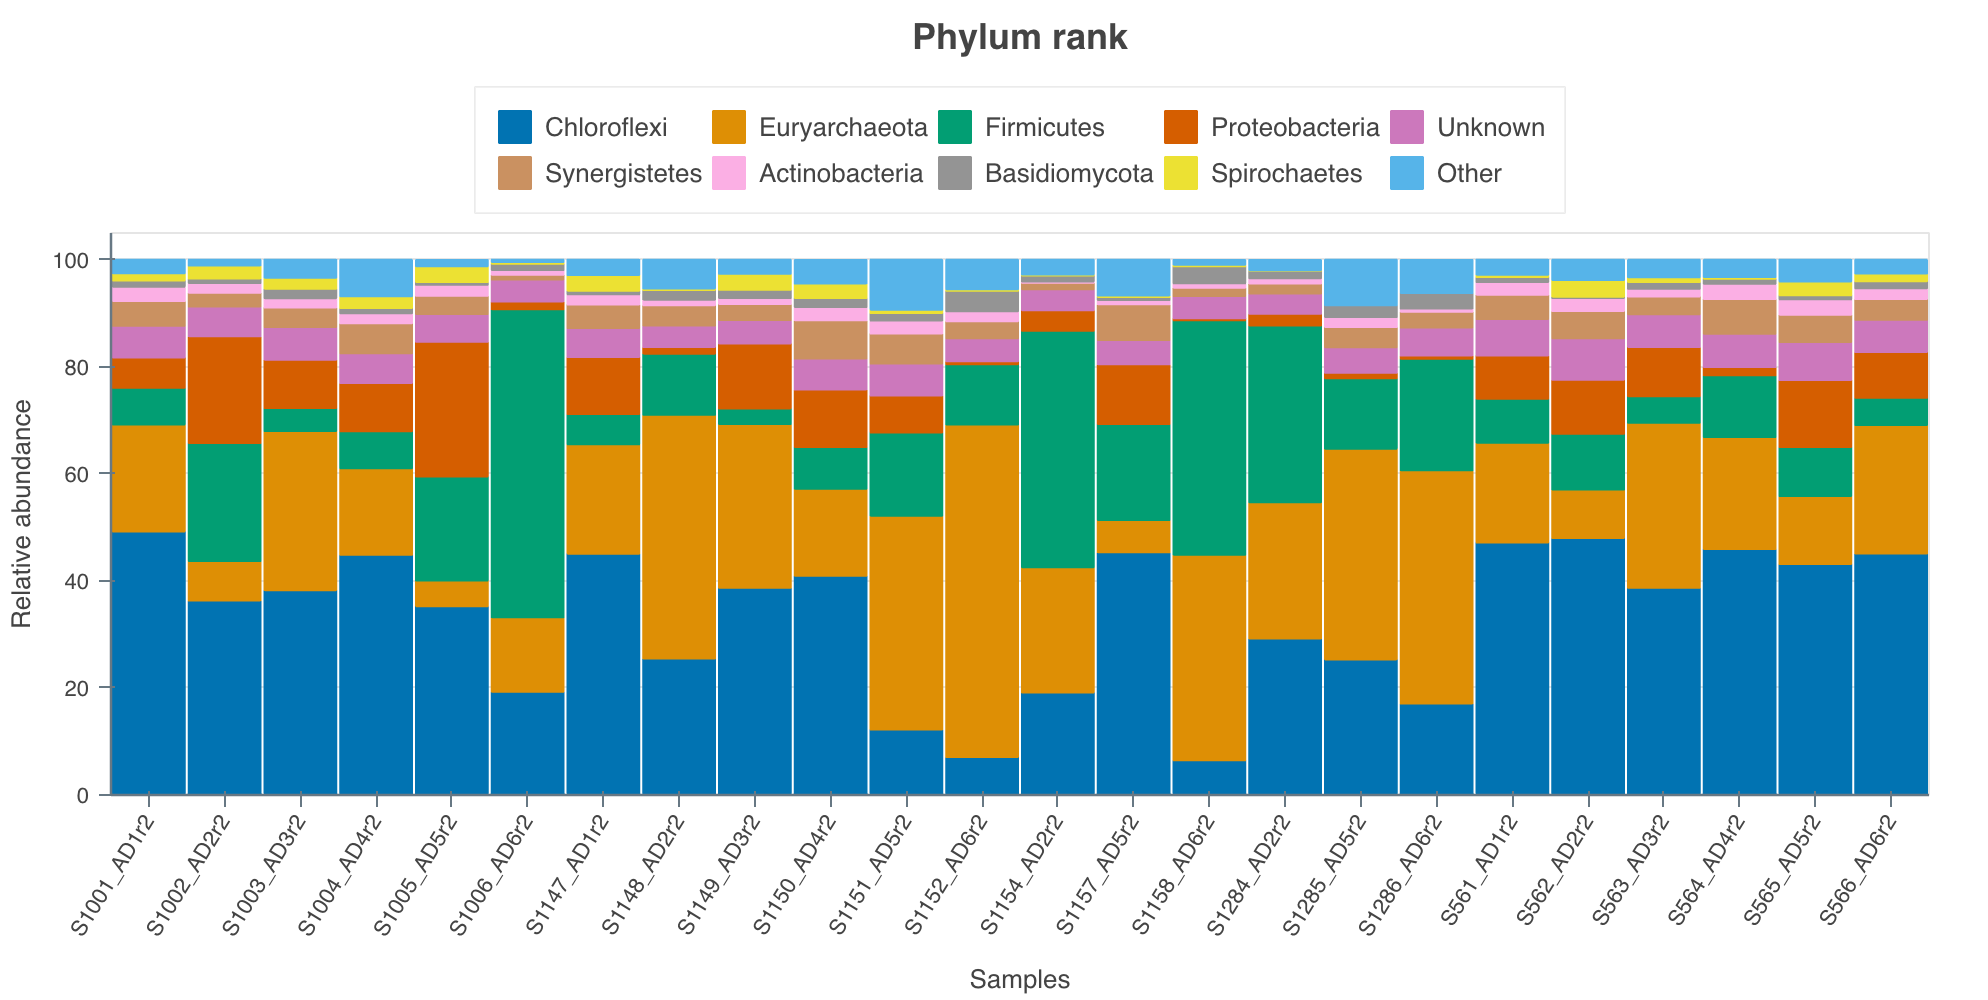
\includegraphics[width=5.20833in,height=\textheight]{./img/results2.png}\\
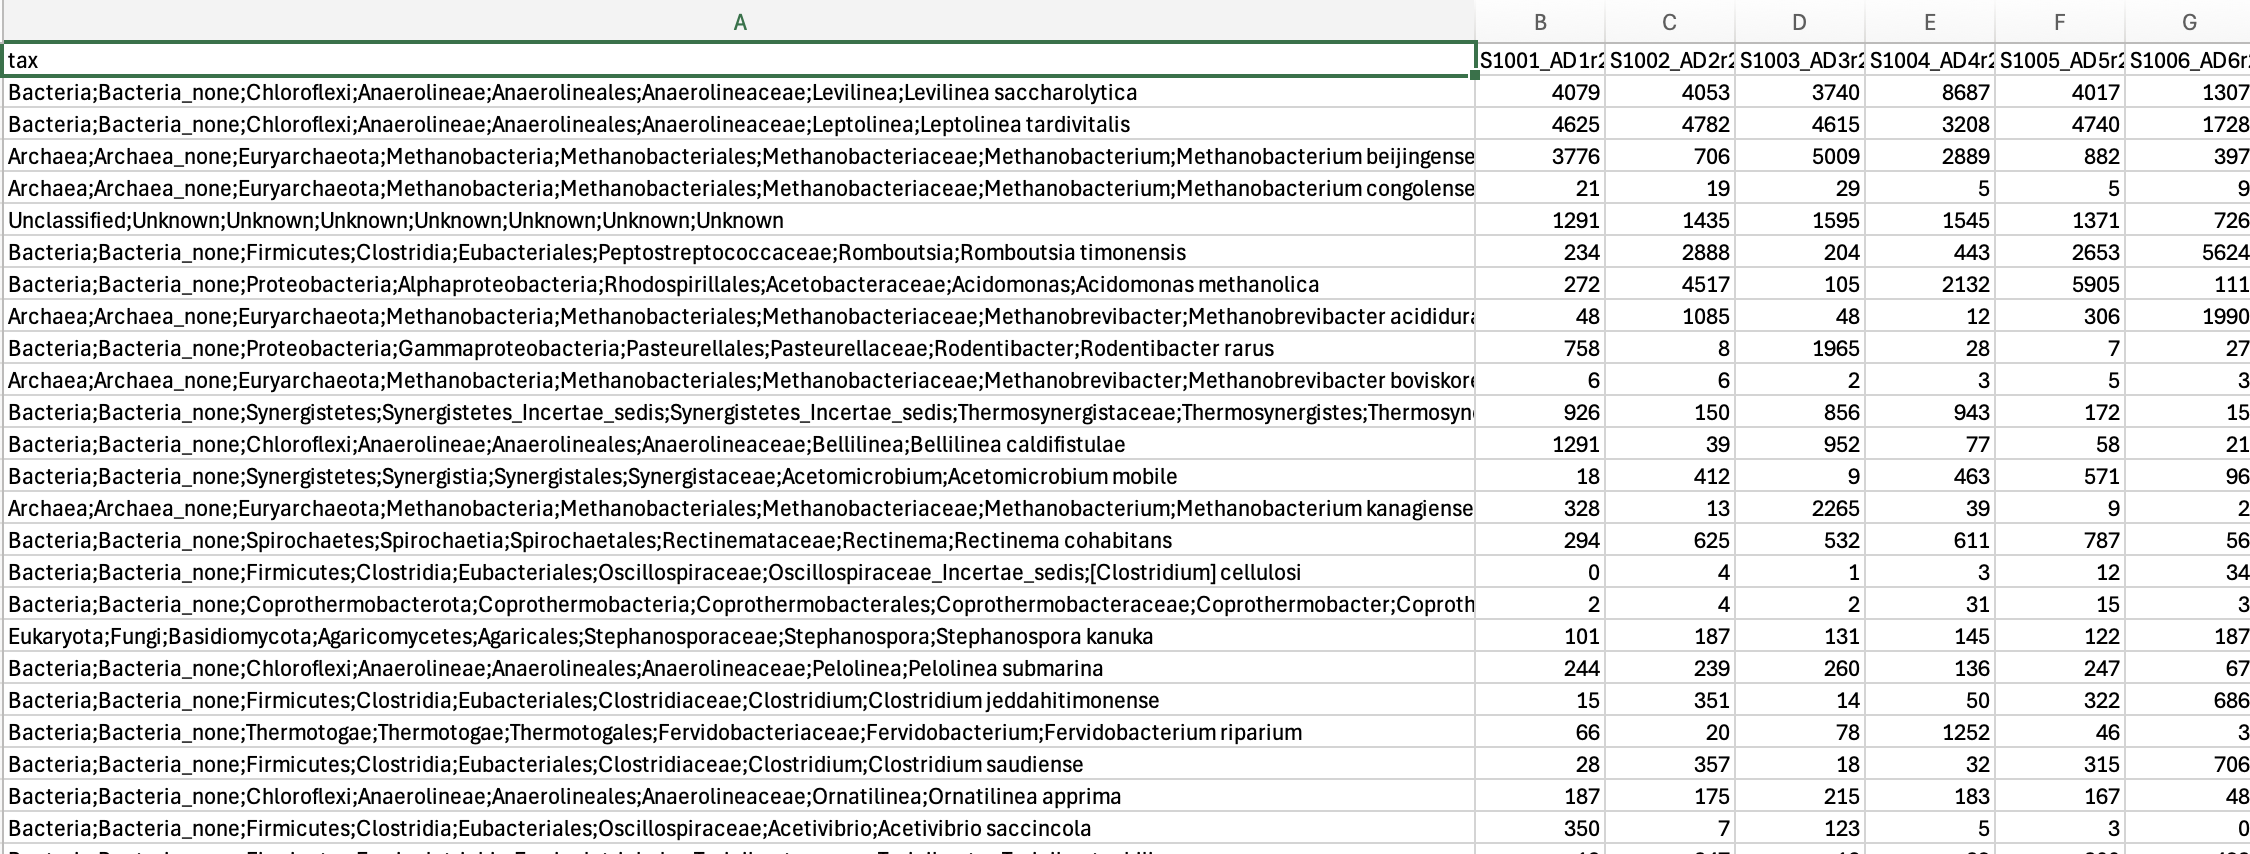
\includegraphics[width=5.20833in,height=\textheight]{./img/results3.png}

  \bibliography{book.bib,packages.bib}

\end{document}
